% Graduation project book — Predictive Maintenance for OBD-II Engine Faults
% AAST College of Engineering and Technology, Computer Engineering Department
% Build: pdflatex main && bibtex main && pdflatex main && pdflatex main
\documentclass[12pt,a4paper]{article}

\usepackage[a4paper,margin=2.5cm]{geometry}
\usepackage{graphicx}
\usepackage{booktabs}
\usepackage{longtable}
\usepackage{acronym}
\usepackage{float}
\usepackage{amsmath}
\usepackage{subcaption}
\usepackage{listings}
\usepackage{xcolor}
\usepackage{setspace}
\usepackage{fancyhdr}
\usepackage{titlesec}
\usepackage[hidelinks]{hyperref}

\graphicspath{{figures/}}

% ── Typography and layout ────────────────────────────────────────────────────
\onehalfspacing
\setlength{\parskip}{4pt}

\titleformat{\section}{\Large\bfseries}{\thesection}{0.8em}{}
\titleformat{\subsection}{\large\bfseries}{\thesubsection}{0.7em}{}
\titleformat{\subsubsection}{\normalsize\bfseries}{\thesubsubsection}{0.6em}{}

\setlength{\headheight}{14pt}
\pagestyle{fancy}
\fancyhf{}
\fancyhead[L]{\small Predictive Maintenance for OBD-II Engine Faults}
\fancyhead[R]{\small\thepage}
\renewcommand{\headrulewidth}{0.3pt}

% ── Code listings ─────────────────────────────────────────────────────────────
\definecolor{codebg}{RGB}{247,247,245}
\definecolor{codecomment}{RGB}{90,120,90}
\definecolor{codekw}{RGB}{0,70,160}
\definecolor{codestr}{RGB}{150,60,20}

\lstdefinestyle{pystyle}{
  language=Python,
  basicstyle=\ttfamily\scriptsize,
  backgroundcolor=\color{codebg},
  commentstyle=\color{codecomment}\itshape,
  keywordstyle=\color{codekw}\bfseries,
  stringstyle=\color{codestr},
  numbers=left,
  numberstyle=\tiny\color{gray},
  numbersep=6pt,
  breaklines=true,
  breakatwhitespace=true,
  postbreak=\mbox{\textcolor{gray}{$\hookrightarrow$}\space},
  frame=single,
  framerule=0.2pt,
  showstringspaces=false,
  tabsize=4,
  captionpos=b,
  inputencoding=utf8,
  extendedchars=true,
  literate={°}{{\textdegree}}1 {±}{{$\pm$}}1 {→}{{$\to$}}1 {←}{{$\leftarrow$}}1
           {−}{{$-$}}1
           {≈}{{$\approx$}}1 {≤}{{$\le$}}1 {≥}{{$\ge$}}1 {σ}{{$\sigma$}}1
           {Δ}{{$\Delta$}}1 {×}{{$\times$}}1 {—}{{---}}1 {–}{{--}}1
           {‘}{{`}}1 {’}{{'}}1 {“}{{``}}1 {”}{{''}}1 {…}{{...}}3 {│}{{|}}1
           {├}{{|-}}2 {└}{{|-}}2 {─}{{-}}1 {∞}{{$\infty$}}1 {≠}{{$\ne$}}1
           {œ}{{oe}}1 {á}{{\'a}}1 {ã}{{\~a}}1 {é}{{\'e}}1 {ö}{{\"o}}1,
}
\lstdefinestyle{ktstyle}{
  style=pystyle,
  language=Java,   % closest built-in lexer for Kotlin
  morekeywords={fun,val,var,object,data,when,companion,override,lateinit,init},
}

% ── Acronyms convenience ─────────────────────────────────────────────────────
\newcommand{\projecttitle}{Predictive Maintenance for OBD-II Engine Faults}

\begin{document}

% ═══════════════════ FRONT MATTER ═══════════════════
% ─────────────────────────── COVER PAGE ───────────────────────────
\begin{titlepage}
\centering
\vspace{-0.8cm}

\includegraphics[width=3.2cm]{aast.png}\par
\vspace{0.4cm}
{\large\bfseries Arab Academy for Science, Technology and Maritime Transport\par}
\vspace{0.4cm}
{\normalsize College of Engineering and Technology\par}
{\normalsize Computer Engineering Department\par}
\vspace{1.2cm}
{\normalsize B.Sc.\ Final Year Project\par}
\vspace{1.8cm}
{\LARGE\bfseries \projecttitle\par}
\vspace{2.2cm}
{\normalsize\bfseries Presented by:\par}
\vspace{0.4cm}
\begin{tabular}{ll}
Omar Hossam Eldin Mohamed Hafez & Reg.\ No.\ 20101737\\
Mohamed Sameh Mohamed Mohamed El Bassuni & Reg.\ No.\ 18100896\\
Mohamed Mohamed Talaat Abokhatwa & Reg.\ No.\ 12103172\\
Ahmed Abdelaal Saad & Reg.\ No.\ 16101027\\
Adam Mohamed Ibrahim & Reg.\ No.\ 20101978\\
\end{tabular}
\vspace{1.8cm}

{\normalsize\bfseries Supervised by:\par}
\vspace{0.4cm}
{\normalsize Yahia Elderiny\par}
{\normalsize Rania Kadry\par}
\vfill
{\normalsize July --- 2026\par}
\end{titlepage}

\pagenumbering{roman}
\setcounter{page}{2}

% ─────────────────────────── DECLARATION ───────────────────────────
\clearpage
\section*{Declaration}
\addcontentsline{toc}{section}{Declaration}

I hereby certify that this report, which I am now submitting for evaluation on
the study program leading to the award of Bachelor of Science in Computer
Engineering, is all my own work and contains no plagiarism. I comply with the
following terms when submitting this report:

Any text, diagrams or other material copied from other sources (including, but
not limited to, books, journals, and the internet) have been clearly
acknowledged and cited, followed by the reference number used, either in the
text or in a footnote/endnote. The details of the used references that are
listed at the end of the report conform to the referencing style dictated by
the final year project template and are, to my knowledge, accurate and
complete.

I have read the sections on referencing and plagiarism in the final year
project template. I understand that plagiarism can lead to a reduced or fail
grade, in serious cases, for the Graduation Project course.

\vspace{0.8cm}
\noindent
\begin{tabular}{@{}p{0.48\textwidth}p{0.48\textwidth}@{}}
\textbf{Student name:} Omar Hossam Eldin Mohamed Hafez & \textbf{Student name:} Mohamed Sameh Mohamed Mohamed El Bassuni\\
Registration number: 20101737 & Registration number: 18100896\\
Signed: \rule{3cm}{0.3pt} & Signed: \rule{3cm}{0.3pt}\\
Date: \rule{3cm}{0.3pt} & Date: \rule{3cm}{0.3pt}\\[0.6cm]
\textbf{Student name:} Mohamed Mohamed Talaat Abokhatwa & \textbf{Student name:} Ahmed Abdelaal Saad\\
Registration number: 12103172 & Registration number: 16101027\\
Signed: \rule{3cm}{0.3pt} & Signed: \rule{3cm}{0.3pt}\\
Date: \rule{3cm}{0.3pt} & Date: \rule{3cm}{0.3pt}\\[0.6cm]
\textbf{Student name:} Adam Mohamed Ibrahim & \\
Registration number: 20101978 & \\
Signed: \rule{3cm}{0.3pt} & \\
Date: \rule{3cm}{0.3pt} & \\
\end{tabular}

% ─────────────────────────── PROJECT SUMMARY ───────────────────────────
\clearpage
\section*{Senior Project Summary Report}
\addcontentsline{toc}{section}{Senior Project Summary Report}

\begin{center}
Arab Academy for Science, Technology and Maritime Transport\\
College of Engineering and Technology --- Department of Computer Engineering\\
Academic Year: 2025/2026 \qquad Semester: 10
\end{center}

\renewcommand{\arraystretch}{1.3}
\begin{longtable}{@{}p{0.24\textwidth}p{0.72\textwidth}@{}}
\toprule
\textbf{Project title} & \projecttitle\\
\midrule
\textbf{Supervisor(s)} & Yahia Elderiny; Rania Kadry\\
\midrule
\textbf{Team members} &
Omar Hossam Eldin Mohamed Hafez --- 20101737\newline
Mohamed Sameh Mohamed Mohamed El Bassuni --- 18100896\newline
Mohamed Mohamed Talaat Abokhatwa --- 12103172\newline
Ahmed Abdelaal Saad --- 16101027\newline
Adam Mohamed Ibrahim --- 20101978\\
\midrule
\textbf{Project deliverables} &
A physics-constrained fault injection engine for OBD-II time series; a
six-class XGBoost fault classifier with SHAP explanations; a PID forecaster
and one-class anomaly detector; an Android data-collection app (OBD-LOG); a
Streamlit dashboard with an end-of-read health report; and a documented
protocol for future real-fault data collection.\\
\midrule
\textbf{Description} &
The system reads live engine sensor data through the standard OBD-II port at
1\,Hz, converts 60-second windows into 83 vehicle-agnostic features, and
classifies the engine state into healthy, cold-start, or one of four
developing fault classes (vacuum leak, fuel delivery, coolant sensor,
throttle sensor). Because no public real-fault OBD-II dataset exists at this
sample rate, training data is produced by injecting physically plausible
fault signatures into 84.5 hours of real healthy driving data. The pipeline
transfers across vehicles by z-scoring every feature against the target
car's own healthy baseline, and it reports ``Untested'' for any fault whose
required sensor a given car does not expose.\\
\midrule
\textbf{Engineering standards} &
SAE J1979 (OBD-II diagnostic services and PID definitions); ISO 15765-4
(CAN transport for diagnostics); ELM327 AT command set for adapter control;
OBD-II physical ranges used as hard clamps in the injection engine (fuel
trim $\pm$25\,\%, timing advance $\pm$64$^{\circ}$).\\
\midrule
\textbf{Design constraints} &
1\,Hz sampling ceiling of consumer ELM327 adapters (measured 0.37--1.10\,Hz
depending on PID count); Bluetooth Classic SPP throughput; per-vehicle PID
availability (the test Yaris exposes no MAP sensor); no labeled real-fault
data available anywhere at 1\,Hz; laptop-only inference (no cloud
dependency for the demo); all injected values clamped to engine physics.\\
\midrule
\textbf{Project impact} &
Earlier warning of developing engine faults than the check-engine light,
using hardware the average driver can afford (a phone plus a
\$10 adapter); a reusable, physics-grounded methodology for synthesizing
labeled fault data where none exists; an honest evaluation framework that
reports what it cannot test instead of fabricating scores.\\
\midrule
\textbf{Team organization} &
Omar Hossam Eldin Mohamed Hafez --- data pipeline and fault injection.\newline
Mohamed Sameh Mohamed Mohamed El Bassuni --- Android application and vehicle testing.\newline
Mohamed Mohamed Talaat Abokhatwa --- feature engineering and classifier.\newline
Ahmed Abdelaal Saad --- forecaster, anomaly detection, evaluation.\newline
Adam Mohamed Ibrahim --- dashboard, integration, documentation.\\
\midrule
\textbf{Ethics / safety} &
No physical fault was induced on any test vehicle. All driving data was
collected on public roads with the driver's consent, at legal speeds, with
the phone mounted and operated by a passenger. Model outputs are advisory
only; a qualified mechanic must confirm any suspected fault before repair
decisions. The synthetic origin of all fault labels is disclosed in every
result table.\\
\bottomrule
\end{longtable}

\vspace{0.6cm}
\noindent Main Supervisor Signature: \rule{5cm}{0.3pt}

% ─────────────────────────── STUDENTS CONTRIBUTION ───────────────────────────
\clearpage
\section*{Students Contribution}
\addcontentsline{toc}{section}{Students Contribution}

\begin{center}
\projecttitle\\[0.4cm]
Submitted by: Omar Hossam Eldin Mohamed Hafez, Mohamed Sameh Mohamed Mohamed El Bassuni, Mohamed Mohamed Talaat Abokhatwa, Ahmed Abdelaal Saad, Adam Mohamed Ibrahim
\end{center}

\vspace{0.5cm}
\begin{center}
\begin{tabular}{clp{5.5cm}}
\toprule
\textbf{Chapter} & \textbf{Title} & \textbf{Contributors}\\
\midrule
1 & Introduction & Omar Hossam Eldin Mohamed Hafez\newline Adam Mohamed Ibrahim\\
\addlinespace
2 & Literature Survey and Related Work & Mohamed Sameh Mohamed Mohamed El Bassuni\newline Mohamed Mohamed Talaat Abokhatwa\\
\addlinespace
3 & The Proposed System & Omar Hossam Eldin Mohamed Hafez\newline Mohamed Sameh Mohamed Mohamed El Bassuni\newline Mohamed Mohamed Talaat Abokhatwa\\
\addlinespace
4 & Experimental Results and Evaluation & Ahmed Abdelaal Saad\newline Adam Mohamed Ibrahim\\
\addlinespace
5 & Conclusion and Future Work & Ahmed Abdelaal Saad\newline Adam Mohamed Ibrahim\\
\bottomrule
\end{tabular}
\end{center}

% ─────────────────────────── ACKNOWLEDGMENT ───────────────────────────
\clearpage
\section*{Acknowledgment}
\addcontentsline{toc}{section}{Acknowledgment}

We wish to express our sincere gratitude to all those who gave us the
opportunity to make tangible progress in this project.

First and foremost, we thank God Almighty for giving us the strength,
knowledge, ability and opportunity to undertake this work and to persevere
and complete it satisfactorily.

Special appreciation for the supervision, advice and continuous encouragement
goes to our advisors, Yahia Elderiny and Rania Kadry.

We would also like to thank the Arab Academy for Science, Technology and
Maritime Transport for the facilities and support that made this project
possible, and Eron J.\ Maranh\~ao for publishing the carOBD dataset that our
training pipeline is built on.

Last but not least, our heartfelt gratitude goes to our families for their
support throughout the year, and to the long-suffering 2015 Toyota Yaris that
idled through every data-collection session without complaint.

% ─────────────────────────── ABSTRACT ───────────────────────────
\clearpage
\section*{Abstract}
\addcontentsline{toc}{section}{Abstract}

Modern cars continuously report engine sensor data through the standardized
OBD-II port, yet that data is used almost exclusively after a fault has
already tripped a diagnostic trouble code. This project builds a predictive
maintenance system that watches the sensor stream itself and flags a
developing fault before the check-engine light fires. The system reads
14 engine parameters at 1\,Hz, summarizes each 60-second window into 83
vehicle-agnostic features, and classifies the window into healthy,
cold-start, or one of four fault classes: intake vacuum leak, fuel delivery
fault, coolant temperature sensor fault, and throttle position sensor fault.

No public OBD-II dataset with labeled real faults exists at this sample rate,
so we trained on synthetic faults injected into 84.5 hours of real healthy
driving data from the public carOBD corpus --- 129 sessions that we recovered
from an upstream CSV parsing defect which had previously made 120 of them
appear corrupt. The injection engine is physics-constrained: every written
value respects engine causality, from the 1$^{\circ}$C-per-second thermal
inertia of coolant to the short-term-to-long-term fuel trim handoff of a real
adaptive ECU. An XGBoost classifier reaches a leave-one-family-out macro-F1
of 0.977 (worst family 0.958), and we report these numbers explicitly as
synthetic self-consistency scores, not as proof of real-fault detection. On a
real, healthy 2015 Toyota Yaris the deployed pipeline correctly declared the
air-system class Untested (the car has no MAP sensor) and refused to issue a
verdict on insufficient evaluable data --- behavior we argue is an
engineering contribution in itself, because an earlier version of the same
pipeline confidently reported a 97\,\% air-system fault on the same healthy
car. The system ships with an Android data-collection app, a live Streamlit
dashboard, and a documented protocol for the real-fault recordings that would
convert the synthetic validation into field validation.

% ─────────────────────────── TOC / LOF / LOT ───────────────────────────
\clearpage
\tableofcontents
\clearpage
\listoffigures
\addcontentsline{toc}{section}{List of Figures}
\listoftables
\addcontentsline{toc}{section}{List of Tables}

% ─────────────────────────── ACRONYMS ───────────────────────────
\clearpage
\section*{List of Acronyms}
\addcontentsline{toc}{section}{List of Acronyms}

\begin{acronym}[XGBoost]
  \acro{OBD-II}{On-Board Diagnostics, second generation --- the standardized
    vehicle diagnostic interface mandated on passenger cars since 1996}
  \acro{PID}{Parameter ID --- one addressable sensor or computed value in the
    OBD-II protocol (e.g.\ 0x0C = engine RPM)}
  \acro{ELM327}{The de-facto standard microcontroller that bridges the OBD-II
    bus to a serial (Bluetooth/USB) link using AT commands}
  \acro{ECU}{Engine Control Unit --- the embedded computer that manages
    fueling, ignition and emissions}
  \acro{MAF}{Mass Air Flow sensor --- measures intake airflow directly}
  \acro{MAP}{Manifold Absolute Pressure sensor --- measures intake manifold
    pressure; the airflow reference on speed-density engines}
  \acro{XGBoost}{eXtreme Gradient Boosting --- a gradient-boosted decision
    tree library}
  \acro{SHAP}{SHapley Additive exPlanations --- a game-theoretic method for
    attributing a model prediction to its input features}
  \acro{ML}{Machine Learning}
  \acro{LOFO}{Leave-One-Family-Out cross-validation (holding out an entire
    session family, e.g.\ all idle recordings)}
  \acro{LOSO}{Leave-One-Session-Out cross-validation}
  \acro{LTFT}{Long-Term Fuel Trim --- the ECU's learned, persistent fuel
    correction, in percent}
  \acro{STFT}{Short-Term Fuel Trim --- the ECU's fast, oscillating fuel
    correction, in percent}
  \acro{DTC}{Diagnostic Trouble Code --- the standardized fault code that
    turns on the check-engine light}
  \acro{API}{Application Programming Interface}
  \acro{CSV}{Comma-Separated Values file format}
  \acro{RPM}{Revolutions Per Minute (engine speed)}
  \acro{IAT}{Intake Air Temperature}
  \acro{TPS}{Throttle Position Sensor}
  \acro{APK}{Android Package --- the installable Android application format}
  \acro{BOM}{Byte Order Mark --- a Unicode signature at the start of a text file}
  \acro{Kafka}{Apache Kafka --- a distributed event-streaming platform}
  \acro{REST}{REpresentational State Transfer --- an HTTP API architectural style}
\end{acronym}
\clearpage


% ═══════════════════ CHAPTERS ═══════════════════
\pagenumbering{arabic}
\setcounter{page}{1}

\section{Introduction}
\label{ch:intro}

\subsection{Overview}

Every passenger car built since the mid-1990s carries a diagnostic socket
under its dashboard. Through that socket --- the OBD-II port --- the engine
control unit (ECU) will answer questions about itself once per second:
engine speed, coolant temperature, how much fuel correction it is currently
applying, how far the throttle plate is open, and dozens more. A ten-dollar
ELM327 Bluetooth adapter turns any phone into a reader for this stream.
The data is there, in every car, all the time.

What the industry does with that stream is mostly reactive. The ECU compares
individual sensors against fixed thresholds, and when one is crossed for long
enough, it stores a diagnostic trouble code (DTC) and lights the check-engine
lamp. By that point the fault is established. The slow drift that preceded it
--- a fuel trim creeping upward for weeks as an injector clogs, an idle speed
rising a little as a vacuum line cracks --- is visible in the sensor stream
long before any threshold trips, but nothing in the standard diagnostic chain
looks for it.

We built a system that looks for it. The system ingests the 1\,Hz OBD-II
stream, summarizes each 60-second window of driving into a feature vector,
and classifies the engine's state into healthy, cold-start, or one of four
developing fault classes. It runs on a laptop, takes its data from either a
recorded CSV file or a live Bluetooth adapter, explains each prediction in
terms of the sensors that drove it, and ends every session with a plain
verdict about the engine's health. Alongside the analysis pipeline we built
an Android application, OBD-LOG, that performs the vehicle-side data
collection on real cars.

One fact shapes the entire project, and we state it here rather than bury it:
there is no public dataset of real, labeled engine faults recorded through
OBD-II at 1\,Hz. Nobody has published one. Our models are therefore trained
on \emph{synthetic} faults --- physically grounded modifications injected
into 84.5 hours of real healthy driving data. Chapter~\ref{ch:results}
quantifies exactly what that means for how the results should be read.

\subsection{Problem Statement}

Given a stream of standard OBD-II sensor readings sampled at approximately
1\,Hz from an unmodified passenger car, decide --- within about a minute of
data --- whether the engine is behaving normally, warming up from a cold
start, or exhibiting the early signature of one of four common fault classes:
an intake vacuum leak, a fuel delivery restriction, a stuck coolant
temperature sensor, or a worn throttle position sensor. The decision must
come with an explanation a mechanic can check, must transfer to vehicles the
model has never seen, and must refuse to answer rather than guess when the
target vehicle does not expose the sensors a given fault requires.

Three properties of the setting make this harder than a textbook
classification exercise. The data rate is low: at 1\,Hz, combustion-level
events are invisible, and only slow aggregate signatures survive. The
labels do not exist: healthy public data is plentiful, but labeled fault
data at this rate is not, so the training signal has to be synthesized
without violating engine physics. And the deployment target varies: two cars
expose different PID sets, idle at different speeds, and trim fuel around
different baselines, so a model fitted to one car's raw values fails on the
next car for reasons that have nothing to do with faults.

\subsection{Motivation and Application}

The gap between ``data available'' and ``warning delivered'' is the
motivation. A drivetrain fault that is caught while it is still a drifting
sensor value costs a hose clamp or a sensor swap; the same fault caught at
the DTC stage may have been degrading fuel economy for months, and caught at
the breakdown stage it costs a tow. Fleet operators already pay for
telematics systems that promise early warning, but those systems are
proprietary, and the published research behind them almost never operates on
the 1\,Hz consumer-grade interface that ordinary vehicles actually expose.

Consider the concrete case of a clogging fuel injector. Early, it shows only
as a long-term fuel trim that has crept from its normal few percent to eight
or nine, correcting for a mixture that is running slightly lean. The car
drives fine; the driver notices nothing; no code is stored. Weeks later the
trim saturates at its limit, the mixture goes lean under load, and now there
is a misfire code, a rough idle, and possibly a damaged catalytic converter
downstream. The whole trajectory was visible in one PID from the first week.
A tool that flagged the drift at week one turns a converter and an injector
into just an injector, and turns a roadside stall into a scheduled
appointment. That is the value proposition in a single fault, and three of
our four fault classes tell structurally similar stories.

The intended applications are concrete. A workshop can replay a customer's
recorded drive and get a per-fault verdict with sensor-level evidence. A
student or hobbyist can point the dashboard at a live car and watch the
classifier, the fuel trims, and the SHAP explanation update together. A
fleet, with the future-work pipeline of Section~\ref{sec:future}, could
stream many vehicles into the same scoring backend. In every case the
hardware cost is a phone and an ELM327 adapter --- perhaps fifteen dollars
of equipment reading data the car already computes and publishes for free.

There is also a methodological application that outlives this particular
system. The fault injection engine of Section~\ref{sec:injector} is a
worked answer to a question many practitioners face: how do you train a
detector when the failure data does not exist? Our answer --- inject faults
into real healthy data under hard physical constraints, document every
parameter, and measure how much the scores depend on the injector's own
settings --- is reusable well beyond these four fault classes.

\subsection{Challenges}

The project's difficulties were not where we first expected them. Put
simply, the models were the easy part; the data was not.

\begin{itemize}
  \item \textbf{A corrupted-looking corpus.} Our first audit of the public
    carOBD dataset concluded that 120 of its 129 files contained physically
    impossible sensor values and had to be discarded. The real cause turned
    out to be a single-character CSV parsing defect --- a trailing comma
    that silently shifted every column one position left. Diagnosing this
    took longer than training any model in this report, and
    Section~\ref{sec:dataset} documents it in full.
  \item \textbf{Synthesizing faults without lying about physics.} A naive
    fault injector produces textbook signatures that real ECUs never emit.
    A vacuum leak on a speed-density engine, for example, does \emph{not}
    produce the large fuel-trim swing the textbooks describe, because the
    MAP sensor sees the leak directly and the ECU compensates. Getting each
    of the four fault models to match documented ECU behavior forced us to
    discard and rewrite our first implementations.
  \item \textbf{Evaluation that does not flatter itself.} Windows cut from
    the same drive overlap by up to 50 of their 60 rows. Any split that
    mixes one session's windows across train and test leaks information and
    inflates F1 by 10--20 points. We had to lock session-level splitting in
    as a tested invariant, and we had to accept that our headline numbers
    measure self-consistency with our own injector, not field detection.
  \item \textbf{Cross-vehicle reality.} The training vehicle (Toyota Etios)
    is a speed-density car with a MAP sensor; our test vehicle (Toyota
    Yaris) is MAF-based and reports no MAP at all. The first deployment on
    the healthy Yaris produced a confident, entirely wrong fault alarm, and
    fixing that failure properly reshaped the system's reporting layer.
  \item \textbf{Throughput of consumer hardware.} A real ELM327 clone polls
    7 PIDs at 1.10\,Hz but 21 PIDs at only 0.37\,Hz. Choosing which PIDs
    are worth their cost in sample rate became a design decision with
    measured trade-offs, not a footnote.
\end{itemize}

None of these five were solved by writing more machine learning code. Each
one was a data problem, a physics problem, or a hardware problem first, and
the model only got to be as good as the data underneath it allowed. That
ordering --- fix the data, then fit the model --- turned out to be the
project's actual methodology, even though it was not the one we set out
with in Week~1.

\subsection{Objectives}

\begin{enumerate}
  \item Recover and validate the full 129-session carOBD corpus, with a
    loud, tested guard against the column-shift defect that had hidden
    93\,\% of it.
  \item Build a fault injection engine for four fault classes, in ramp and
    step modes, in which every written value is clamped to engine physics
    and every injection is reproducible from stored parameters.
  \item Design a vehicle-agnostic feature representation --- 83 features
    per 60-second window, z-scored against the source vehicle's own healthy
    baseline --- that lets a model trained on one car run on another.
  \item Train and evaluate a six-class XGBoost classifier under
    session-level and family-level cross-validation, reporting synthetic
    self-consistency scores as exactly that.
  \item Complement the classifier with a per-PID forecaster and a one-class
    anomaly detector, and report honestly where they fail (long-term fuel
    trim forecasting fails).
  \item Build the OBD-LOG Android app for real-vehicle data collection over
    Bluetooth, with tiered PID selection driven by measured poll rates.
  \item Deploy the full pipeline against real recordings from an unseen
    vehicle, and design the reporting layer so that missing sensors produce
    ``Untested'' verdicts rather than fabricated scores.
  \item Deliver a live dashboard that shows the classification, its SHAP
    explanation, physics-based severity, and an end-of-read health report.
\end{enumerate}

\subsection{Ethics}

No physical fault was induced on any vehicle at any point in this project.
Every fault our models were trained on is synthetic, and every real
recording we scored came from a healthy, unmodified car. We considered
inducing a real vacuum leak under supervision and decided against it for
this phase; the documented collection protocol in the repository specifies
how to do it safely if a future team takes that step, with a mechanic
present and abort conditions defined in advance.

All driving data we collected ourselves was recorded on public roads with
the driver's knowledge and consent, at legal speeds, with the phone mounted
and the app operated by a passenger. The carOBD corpus we trained on is
public, published by its author for research use, and credited in
Chapter~\ref{ch:literature} and the references.

The system's outputs are advisory. A classifier label on a dashboard is not
a diagnosis, and the report says so on its face: every end-of-read verdict
carries its caveats in the rendered output, including the synthetic origin
of the training data and the conditions under which the verdict is
unreliable. A qualified mechanic must confirm any suspected fault before a
repair decision is made. We consider the refusal behaviors --- ``Untested''
when a required sensor is absent, ``insufficient data'' when too few windows
are evaluable --- to be ethics features as much as engineering ones, because
the alternative is a tool that manufactures confident false alarms, and we
watched an early version of our own system do exactly that.

\subsection{Report Layout}

Chapter~\ref{ch:literature} surveys prior work on OBD-II diagnostics and
machine learning for predictive maintenance, and identifies the gap this
project fills. Chapter~\ref{ch:system} describes the proposed system:
architecture, the Android data-collection app, the dataset and its recovery,
the fault injection engine, feature engineering, the models, and the
dashboard. Chapter~\ref{ch:results} presents the evaluation methodology and
results, including the real-vehicle deployment and the failures we kept.
Chapter~\ref{ch:conclusion} concludes with limitations, stated plainly, and
a prioritized future-work list. The appendices contain the key source code
listings from both repositories and the full per-class metric tables.

\clearpage
\section{Literature Survey and Related Work}
\label{ch:literature}

\subsection{Overview}

Work relevant to this project falls into three strands: diagnostics built
directly on the OBD-II interface, machine learning for automotive predictive
maintenance in general, and the specific model family (gradient-boosted
trees with attribution methods) that we deploy. Reading across the three
strands, a consistent pattern emerges: the studies with realistic fault data
do not use the consumer OBD-II interface, and the studies on the consumer
interface do not have realistic fault data. Our project sits precisely in
that intersection, which is why the survey below pays as much attention to
each paper's \emph{data source} as to its model.

\subsection{Related Work}

\subsubsection{Diagnostics on the OBD-II interface}

Rimpas et al.~\cite{rimpas2020} logged OBD-II parameters --- fuel trims,
coolant temperature, ignition timing, and airflow among them --- to monitor
vehicle operation and fuel consumption, and discussed how deviations in
individual PIDs indicate specific degradations. Their work confirms the
diagnostic value of exactly the PIDs our system builds features on, but the
analysis is per-parameter and threshold-style. No classifier is trained, and
no labeled faults are used; the interpretation of a drifting trim value is
left to the reading engineer.

Shafi et al.~\cite{shafi2018} built a remote health-monitoring system with
an OBD-II dongle streaming to a phone and applied several classifiers
(decision trees, SVM, k-NN) to detect anomalies in four vehicle subsystems.
Their fault examples, however, come from threshold rules applied to the same
stream the classifiers read --- the labels are derived from the data rather
than from independently verified physical faults. The system demonstrates
the plumbing of phone-based OBD-II ML but not validated fault detection.

The carOBD dataset and its accompanying thesis by
Maranh\~ao~\cite{maranhao_carobd} provide the raw material our project
trains on: 129 sessions of 1\,Hz OBD-II logging from a single Toyota Etios,
covering idle, commute, campus, highway, and long-trip driving. The dataset
contains healthy driving only. To our knowledge no public OBD-II corpus at
this rate contains verified, labeled faults; we searched for one and did not
find it, and this absence is the central constraint the project designs
around.

That absence is structural, not an oversight anyone will quickly correct.
Collecting labeled fault data at scale means deliberately breaking cars, or
waiting for a fleet's worth of them to break naturally while logging
continuously, and then joining the logs to verified repair records. The first is expensive and, done carelessly,
dangerous; the second requires fleet access and years of patience. Whoever
pays for either has a commercial reason to keep the result private. The
public-data vacuum that Theissler et al.\ describe at the field level is, in
other words, structural, and a graduation project cannot fill it by trying
harder. It can only decide how to work honestly inside it, which is the
decision Section~\ref{sec:injector} documents.

\subsubsection{Machine learning for automotive predictive maintenance}

Theissler et al.~\cite{theissler2021} survey machine learning for predictive
maintenance across the automotive industry and catalogue the field's
recurring obstacles: scarce labeled failure data, class imbalance, and the
gap between lab results and fleet deployment. They note explicitly that
run-to-failure data for vehicles is rarely public because it is expensive
and commercially sensitive --- the same wall we hit, met in their survey as
a field-wide condition rather than a local complaint.

Prytz et al.~\cite{prytz2015} predicted compressor repairs in a commercial
truck fleet from logged vehicle data and workshop maintenance records. Their
labels are real --- actual repairs --- but the data source is an OEM fleet
telematics database with service-record joins, not the standardized consumer
port, and the features are aggregated per vehicle-visit rather than
streaming windows. The study demonstrates that drift-before-failure is
learnable in principle, at fleet scale, with access no individual owner has.

Theissler~\cite{theissler2017} addressed the known/unknown fault problem
with ensemble anomaly detection over in-vehicle recordings, arguing that a
detector must handle fault types absent from training. Our two-pillar
design --- a supervised classifier for the four modeled faults plus a
one-class IsolationForest~\cite{liu2008} trained on healthy windows only ---
is a direct application of that argument at consumer-hardware scale.

Vergara et al.~\cite{vergara2023} published EngineFaultDB, a labeled engine
fault dataset with baseline classification results. The faults are real, but
they were produced on a laboratory engine test bench with instrumentation
beyond the OBD-II PID set, sampled under controlled load profiles. We
considered benchmarking against it and declined: a bench dynamometer corpus
and a 1\,Hz road-driving corpus differ in sensors, dynamics, and noise floor
to the point where a comparison table would mislead more than inform.

\subsubsection{Models and attribution}

Gradient-boosted decision trees remain the strongest general-purpose family
for tabular sensor features, and XGBoost~\cite{chen2016} is its standard
implementation; random forests~\cite{breiman2001} provide the natural
bagging baseline. For attribution we use SHAP~\cite{lundberg2017}, whose
TreeExplainer computes exact Shapley values for tree ensembles --- on a
workshop floor, ``LTFT pushed this prediction toward fuel-system by 0.43''
is an explanation a mechanic can act on. The protocol layer underneath the
whole pipeline is standardized by SAE J1979~\cite{saej1979} and
ISO 15765-4~\cite{iso15765}, and our tooling builds on the python-obd
library~\cite{pythonobd}, Streamlit~\cite{streamlit}, and
FastAPI~\cite{fastapi}.

Table~\ref{tab:relwork} lays the surveyed work along the two axes that
decide whether a result transfers to our setting: the realism of its fault
labels and the interface its data came through. The pattern is stark ---
every row has one or the other, never both.

\begin{table}[H]
  \centering
  \caption{Related work along the two axes that matter for our problem:
    fault-label realism and data interface. No surveyed work combines
    verified faults with the 1\,Hz consumer OBD-II interface.}
  \label{tab:relwork}
  \begin{tabular}{lll}
    \toprule
    Work & Fault labels & Data source\\
    \midrule
    Rimpas et al.~\cite{rimpas2020} & None (per-PID thresholds) & Consumer OBD-II\\
    Shafi et al.~\cite{shafi2018} & Derived from the stream & Consumer OBD-II\\
    Prytz et al.~\cite{prytz2015} & Real (repair records) & OEM fleet telematics\\
    Vergara et al.~\cite{vergara2023} & Real (induced) & Bench dynamometer\\
    Theissler~\cite{theissler2017} & Mixed known/unknown & In-vehicle recordings\\
    \textbf{This work} & Synthetic, physics-constrained & Consumer OBD-II, 1\,Hz\\
    \bottomrule
  \end{tabular}
\end{table}

\subsection{Gap Analysis}

Laying the surveyed work side by side exposes four gaps.

\textbf{Realistic faults and consumer hardware do not co-occur.} Bench
studies such as EngineFaultDB~\cite{vergara2023} have verified faults but
non-OBD instrumentation and dynamometer conditions. Fleet studies such as
Prytz et al.~\cite{prytz2015} have real repair labels but proprietary
telematics access. OBD-II studies such as Shafi et al.~\cite{shafi2018}
run on the consumer port but lack independently verified fault labels.
No surveyed work trains and evaluates on the 1\,Hz consumer interface with
trustworthy fault ground truth --- because the data to do so does not
publicly exist.

\textbf{Single-vehicle scope is the norm, and transfer is untested.} The
carOBD corpus is one Etios; EngineFaultDB is one bench engine; most OBD-II
papers instrument one car. Almost none of the surveyed systems state what
happens when the trained model meets a different vehicle --- different
idle speed, different trim baseline, different PID set. In our experience
that encounter is where deployments actually fail.

\textbf{Missing sensors are not handled honestly.} Every surveyed system
assumes its input channels exist. But PID support varies car to car: our
own test vehicle exposes no MAP sensor, the primary channel for one of our
four fault classes. No prior system we found defines what it reports when
the evidence for a fault class is physically absent.

\textbf{Synthetic injection, where used, is not physics-audited.} Adding
offsets or noise to sensor channels is common in anomaly detection
research, but the surveyed automotive works do not constrain injected
values to ECU causality --- fuel trims that lead instead of react, coolant
that jumps faster than thermal mass allows, MAP exceeding barometric
pressure. Models trained on physically impossible signatures learn
artifacts that no real fault will ever reproduce.

\subsection{How This Project Fills the Gap}

Against the first gap, we accept the absence of real-fault data as a design
input rather than pretending otherwise: we train on physics-constrained
synthetic faults injected into real 1\,Hz driving data, we measure how much
the scores depend on the injector's own coefficients (the withheld-parameter
experiment of Section~\ref{sec:evalmethod}), and we label every reported
number as synthetic self-consistency. The deliverable is a detection
algorithm plus a collection protocol, and the report never claims more.

Against the second, every feature is z-scored against the source vehicle's
own healthy baseline (Section~\ref{sec:features}), so the model reasons in
``standard deviations from this car's normal'' rather than raw units, and
the deployed pipeline re-fits that baseline per vehicle. Our evaluation
splits by session and by session \emph{family}, the closest available proxy
for context transfer within a single-vehicle corpus.

Against the third, the pipeline carries an explicit evaluability contract:
each fault class declares the PIDs its primary signature requires, and a
vehicle that lacks them gets ``Untested'' for that class instead of a score
(Section~\ref{sec:dashboard}). Chapter~\ref{ch:results} shows this contract
working on a real MAF-based car.

Against the fourth, the injection engine enforces hard physical clamps and
documented ECU response dynamics --- including the speed-density vacuum-leak
behavior and the STFT-to-LTFT handoff --- with every injection reproducible
from stored parameters (Section~\ref{sec:injector}). The physics arguments
are written into the source alongside the code they constrain.

\clearpage
\section{The Proposed System}
\label{ch:system}

\subsection{System Architecture}
\label{sec:architecture}

Figure~\ref{fig:architecture} shows the system end to end. On the vehicle
side, an ELM327 Bluetooth adapter plugs into the OBD-II port and speaks to
our Android app, OBD-LOG, over a Bluetooth Classic serial link. The app
polls the ECU, decodes each PID reply, and writes timestamped CSV files.
Those files cross to the analysis side, where an adapter layer renames
columns and resamples to a strict 1\,Hz grid, and an inference engine scores
each 60-second window. A Streamlit dashboard renders the live state and, at
the end of a recording, an overall health report.

\begin{figure}[H]
  \centering
  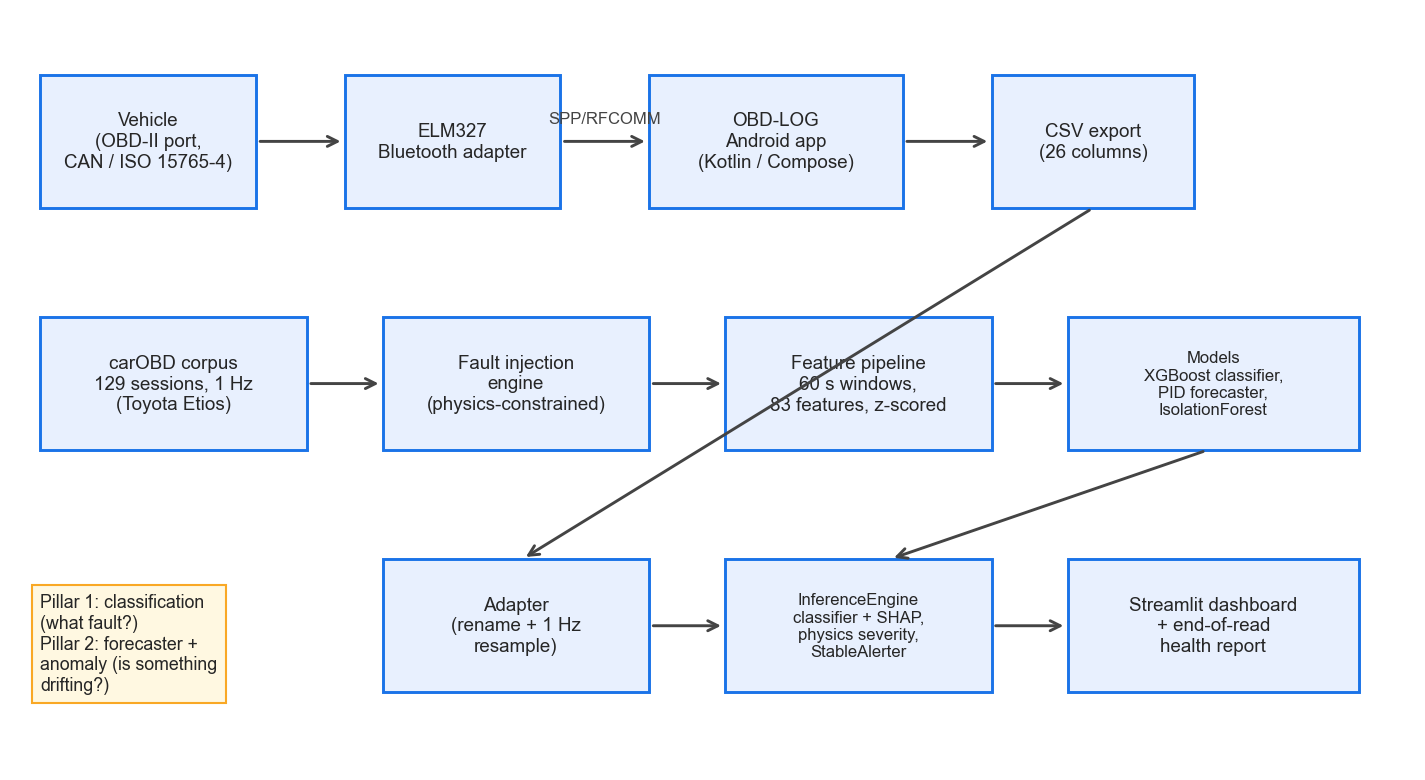
\includegraphics[width=\textwidth]{fig_architecture.png}
  \caption{System architecture. The top row is the acquisition path on the
    vehicle; the middle row is the training pipeline built on the carOBD
    corpus; the bottom row is the inference path that scores recordings and
    drives the dashboard.}
  \label{fig:architecture}
\end{figure}

The analysis side is deliberately organized as two pillars that answer two
different questions. Pillar~1 is the supervised six-class XGBoost classifier:
\emph{if} something is wrong, \emph{which} of the modeled faults does this
window look like? Pillar~2 is the pair of unsupervised safety nets --- a
per-PID forecaster whose prediction residuals flag drift, and a one-class
IsolationForest that scores how far the current window sits from the healthy
manifold. Pillar~2 exists because Pillar~1 can only name faults it was
trained on; a real engine is under no obligation to fail in one of our four
ways.

Both pillars consume the same feature pipeline and the same per-vehicle
baseline normalization, so a single calibration step (recording a few
minutes of healthy driving) adapts the whole stack to a new car. Everything
runs offline on a laptop; the live demo needs no network connection.

\subsection{Data Collection --- the OBD-LOG Android App}
\label{sec:android}

Public data covers the training side, but deploying against real cars
required our own acquisition tool, so we wrote one. OBD-LOG is a native
Android app in Kotlin with a Jetpack Compose / Material~3 interface. It
connects to any ELM327-compatible adapter over Bluetooth Classic
(SPP/RFCOMM), initializes it with the standard AT sequence (reset, echo off,
linefeeds off, spaces off, automatic protocol detection), asks the ECU which
PIDs it actually supports via the 0100/0120/0140 support bitmasks, and then
polls the supported set in a round-robin loop, appending one CSV row per
sweep. The full logger and PID-table sources are reproduced in
Appendix~\ref{app:android}. Our test vehicle throughout was a 2015 Toyota
Yaris, which talks ISO 15765-4 CAN~\cite{iso15765}.

The app's central design decision is a three-tier PID list, because polling
is serial: every extra PID costs sample rate for all of them. Tier~1
(``Core'') carries the nine highest fault-signal channels --- RPM, load,
MAP, MAF, coolant, intake air temperature, both fuel trims, and timing
advance. Tier~2 (``Extended'') adds context: speed, throttle, commanded
equivalence ratio, module voltage, barometric pressure. Tier~3 (``Full'')
adds the remaining niche channels through to catalyst temperatures, kept
mainly for throughput testing. We measured the trade-off directly on the
Yaris at parked idle, and Table~\ref{tab:pollrate} shows why the tiers
exist: tripling the PID count costs two-thirds of the sample rate.

\begin{table}[H]
  \centering
  \caption{Measured poll rate versus polled PID count (2015 Toyota Yaris,
    ELM327 Bluetooth clone, parked idle).}
  \label{tab:pollrate}
  \begin{tabular}{lccc}
    \toprule
    Capture mode & PIDs polled & Measured rate & Rows in test capture\\
    \midrule
    Core     & 7  & 1.10\,Hz & 124\\
    Extended & 12 & 0.64\,Hz & 121\\
    Full     & 21 & 0.37\,Hz & 65\\
    \bottomrule
  \end{tabular}
\end{table}

The three captures in Table~\ref{tab:pollrate} were all successful
end-to-end runs: connect, init, detect, log, export. They also produced the
project's single most consequential hardware finding: the Yaris returned
\texttt{NO DATA} for PID 010B on every request. The car has no MAP sensor
--- it is a MAF-based engine --- so the \texttt{INTAKE\_MANIFOLD\_PRESSURE}
column is empty in every capture. We added MAF (PID 0110) to the Core tier
in response, and Section~\ref{sec:dashboard} describes how the analysis side
was redesigned to survive exactly this kind of per-vehicle sensor absence.

Each CSV carries 26 columns: \texttt{timestamp\_ms} (epoch milliseconds),
\texttt{datetime} (human-readable), and all 24 defined PIDs in fixed order.
Unpolled or unsupported PIDs are written as empty cells rather than dropped,
so every capture has an identical schema regardless of mode --- a property
the downstream adapter relies on. The interface is four screens behind a
navigation drawer: \emph{Dashboard} (connection control, live values, start/stop
logging), \emph{Logs} (recorded files with share/export), \emph{Diagnostics}
(the raw ELM327 init log and support-detection output, which proved
invaluable against clone adapters), and \emph{About}.

One improvement is conspicuously absent and deliberately listed as future
work: a session-label text field written into the CSV, so a recording can
declare itself ``baseline'' or ``induced fault X'' without an external
notebook. It is a one-line UI change, and it is exactly what the real-fault
collection protocol will need.

\subsection{Dataset --- carOBD}
\label{sec:dataset}

Training data comes from carOBD~\cite{maranhao_carobd}, a public corpus of
1\,Hz OBD-II logs from a single Toyota Etios 2014 recorded through a
Carloop (ELM327-compatible) device across 27 PIDs. The corpus spans five
session families: parked idle (\texttt{idle}, 47 files), a recurring
work--home commute (\texttt{live}, 39), highway-style driving
(\texttt{drive}, 13), long trips (\texttt{long}, 12), and low-speed
university-campus driving (\texttt{ufpe}, 18). After the parsing repair
described next, the working corpus is 129 files, 304{,}299 rows, roughly
84.5 hours of driving.

\subsubsection{The trailing-comma discovery}
\label{sec:trailingcomma}

Our Week-1 audit checked every file against physical bounds for four
signature PIDs and produced an alarming result: 120 of 129 files carried
timing-advance values between 30$^{\circ}$ and 776$^{\circ}$, where the
OBD-II encoding cannot exceed $\pm$64$^{\circ}$~\cite{saej1979}. We
initially concluded the files used inconsistent logger firmware and cut the
working set to the 9 clean files --- about 4.4 hours of data --- which is
painfully little for a six-class problem.

The real cause was one character per line. The affected files end every data
row with a trailing comma, so each row parses to 28 fields against 27 header
names. Given that mismatch, \texttt{pandas.read\_csv} silently resolves the
difference by promoting the first column to the row index --- and thereby
shifts \emph{every} column one position left. Coolant temperature reads
fuel-trim values. Timing advance reads catalyst temperature, which is
exactly why we saw ``timing'' of 300--776$^{\circ}$: those are plausible
catalyst temperatures in $^{\circ}$C. The data was never corrupt. The parse
was.

\begin{figure}[H]
  \centering
  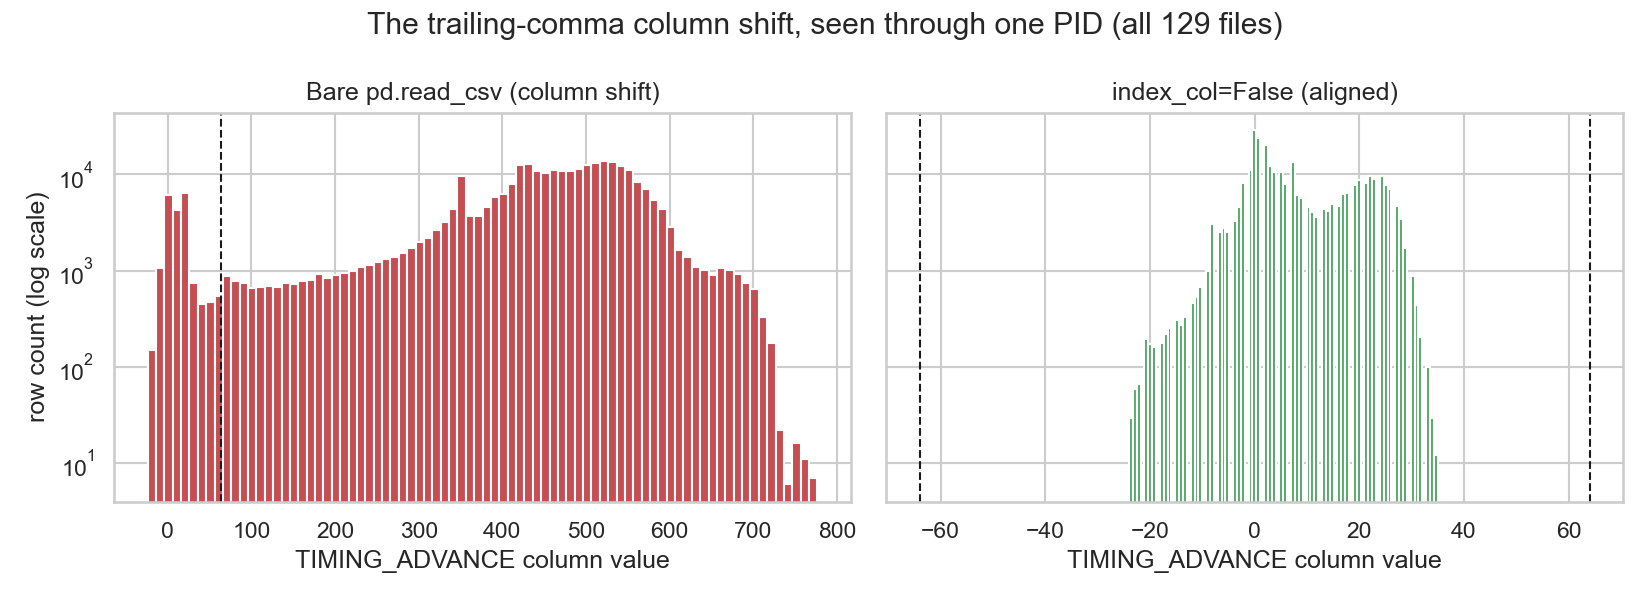
\includegraphics[width=\textwidth]{fig_timing_fix.png}
  \caption{The column-shift defect seen through one PID. Left: under a bare
    \texttt{read\_csv}, the TIMING\_ADVANCE column contains a large
    population far outside the $\pm$64$^{\circ}$ OBD-II bound (dashed
    lines), peaking at 776.6$^{\circ}$ --- catalyst temperatures wearing the
    wrong column name. Right: with \texttt{index\_col=False} the same files
    yield $-24^{\circ}$ to $+35^{\circ}$, entirely inside the physical
    range. Note the logarithmic count axis.}
  \label{fig:timingfix}
\end{figure}

The repair has three parts, and all three stay in the codebase. First,
\texttt{index\_col=False} tells the parser never to promote a column, which
aligns all 27 columns in every file. Second, a numeric coercion pass
converts stray non-numeric cells (one file hides a lone space character in
the intake-air-temperature column) to missing values instead of letting one
bad cell change a whole column's type. Third --- the part we consider
non-negotiable --- a physical-bounds guard re-checks the four signature PIDs
on every load and raises a loud error on violation, so any future
misalignment fails at the loader instead of entering training as scrambled
``healthy'' data. A regression test locks the guard in place. The fix took
the usable corpus from 9 files ($\sim$4.4\,h) to 129 files
($\sim$84.5\,h), a 19$\times$ expansion, and Figure~\ref{fig:timingfix} is
the before/after evidence.

Frankly, this bug taught us more about data engineering than any lecture
could: the failure mode was silent, the symptom appeared two layers away
from the cause, and the wrong-but-plausible explanation (bad firmware)
survived for weeks because it fit the evidence we had.

\subsubsection{Working PID set}

Four of the 27 channels are dead in this corpus and are dropped at load
time: the commanded equivalence ratio is always zero (the Etios ECU does not
report it), the two MIL counters are always zero (healthy car, lamp never
lit), and warm-ups-since-codes-cleared is pinned at the OBD sentinel 255.
Of the remaining channels, 14 form the working feature set
(\texttt{USEFUL\_PIDS}): RPM, speed, throttle, engine load, coolant
temperature, both fuel trims, MAP, both accelerator-pedal channels,
commanded throttle, intake air temperature, timing advance, and control
module voltage.

\subsection{Fault Injection Engine}
\label{sec:injector}

The injection engine is the project's most technically serious contribution,
and it exists for a blunt reason: the faults we want to detect are not for
sale in any public dataset, so we had to write them --- without writing
physics fiction. The governing rule, enforced in code, is that the engine
never emits a sensor value that violates engine causality. Fuel trims are
clamped to the OBD-II $\pm$25\,\% range, coolant may not change faster than
1$^{\circ}$C per second (thermal inertia), MAP may not exceed barometric
pressure on a naturally aspirated engine, throttle stays within
0--100\,\%, and timing stays within its normal $-10^{\circ}$ to
$+40^{\circ}$ envelope. The full source is Appendix~\ref{app:python}
Listing~\ref{lst:injector}.

Each of the four fault models encodes a specific mechanical argument.

\textbf{Air system (vacuum leak).} Our first implementation followed the
textbook: a leak means unmetered air, so short-term fuel trim swings
strongly positive. We rejected that model after checking it against the
engine we actually train on. The Etios reports MAP, load, and barometric
pressure but no MAF --- it is a \emph{speed-density} engine, which computes
airflow \emph{from} manifold pressure. On such an engine the MAP sensor
measures the post-leak pressure directly, the ECU recomputes airflow from
it, and fuel largely self-compensates; service literature for MAP-only
engines describes a slightly raised idle as often the only symptom. The
corrected model therefore raises idle RPM (the leak behaves like a
cracked-open throttle blade, about 15\,rpm per unit of leak magnitude,
clamped to a 1{,}500\,rpm idle ceiling), raises idle MAP slightly, raises
calculated load slightly, and applies only a small, idle-gated fuel-trim
bump that washes out entirely off idle. Every effect is weighted by an
idle factor that goes to zero as load rises, because a leak that is 20\,\%
of airflow at idle is noise at wide-open throttle.

\textbf{Fuel system (injector clog / low rail pressure).} Less fuel per
spray cycle produces a chronic lean condition that the ECU corrects. The
detail that matters --- and that a naive injector gets wrong --- is the
division of labor between the two trims. Short-term trim is the fast
corrector: it \emph{leads} during the developing fault. Long-term trim is
the learned correction: it integrates upward and \emph{holds}. Once the
fault stops developing, STFT bleeds back toward zero (still oscillating)
over roughly a 60-second constant while LTFT retains the full offset. Our
\texttt{\_steady\_state\_trim} helper implements exactly this handoff, so a
developed fuel fault presents as high LTFT with near-zero mean STFT --- the
relationship a real adaptive ECU produces. MAP is deliberately left
untouched: an injector restricts fuel, not air, and that untouched MAP is
what separates a fuel fault from an air fault in feature space. A small
idle-only RPM jitter models the roughness of an unevenly fed engine.

\textbf{Coolant temperature sensor (stuck cold).} The reported temperature
drifts toward a stuck value (default 42$^{\circ}$C), with the
1$^{\circ}$C-per-second clamp applied sample by sample so the trajectory
respects thermal inertia even in step mode. The ECU consequences follow:
timing is retarded in proportion to the perceived cold deficit (up to
5$^{\circ}$), and --- the consequence our first version missed entirely ---
the ECU holds cold-start enrichment because it believes the engine never
warmed up, so once closed-loop operation is reached the fuel trims go
\emph{negative} (rich), delivered through the same STFT-to-LTFT handoff. A
stuck-cold sensor without the rich bias would be a signature no real car
produces.

\textbf{Throttle position sensor (potentiometer wear).} The reported
throttle angle drifts multiplicatively (default full-ramp factor 1.35), but
only on rows where the accelerator pedal exceeds 10\,\% --- a worn
potentiometer track is not loaded at closed throttle, so idle rows stay
clean. The commanded-throttle channel is deliberately left unchanged, which
makes reported-versus-commanded divergence a second, independent signal on
top of the throttle-to-pedal ratio.

Two properties hold across all four models. Degradation is a \emph{ramp}:
severity rises linearly from zero at a configurable onset (default 40\,\%
into the session) over a configurable width (default 15\,\%), then holds
--- modeling gradual wear, with step mode as the one-row limiting case.
And every injection is reproducible: the random seed, onset index, ramp
length, magnitude, and noise level are stored in the output's metadata, so
any training window can be traced to exactly the parameters that produced
it.

One threat looms over all of this, and we measured it instead of waving at
it. The classifier learns to invert the injector; the injector defines the
answer key. If the model merely memorizes our coefficients, its scores are
meaningless for any fault we did not author. The withheld-configuration
experiment in Section~\ref{sec:evalmethod} trains on one full parameter
configuration and tests on a shifted one --- different magnitudes, onset,
ramp width, and noise --- and the observed macro-F1 gap is 0.033. Small,
but not zero, and we report every synthetic score in this book with that
caveat attached: they are a self-consistency floor, not field detection.

\subsection{Feature Engineering}
\label{sec:features}

The 60-second window and 10-second stride are not arbitrary. Sixty seconds
is long enough to capture the slow signatures the faults live in --- a fuel
trim settling to a new level, a coolant curve failing to rise --- while
staying short enough that a driver's state (idling, accelerating, cruising)
is roughly constant across the window, which keeps the regime features
meaningful. The 10-second stride means consecutive windows overlap by 50
seconds, giving a sixfold data-augmentation effect over non-overlapping
windows. That overlap is also precisely why the evaluation of
Section~\ref{sec:evalmethod} must split by session: two windows ten seconds
apart are almost the same window, and letting one train while the other
tests is self-examination, not generalization.

The classifier never sees raw rows. Each 60-second window (stride 10\,s)
is summarized into 83 features in four groups:

\begin{itemize}
  \item \textbf{Per-PID statistics (70).} For each of the 14 working PIDs:
    mean, standard deviation, minimum, maximum, and first-to-last delta.
  \item \textbf{Cross-PID ratios (4).} \texttt{THROTTLE\_TO\_PEDAL\_RATIO}
    (the TPS fault's home signal, computed as the median per-row ratio over
    pedal-active rows only, because the mean ratio explodes at idle);
    \texttt{MAP\_PER\_THROTTLE} (airflow sanity, open-throttle rows only);
    \texttt{FUEL\_TRIM\_DIVERGENCE} ($\mathrm{LTFT} - \mathrm{STFT}$, which
    directly encodes the handoff state); and
    \texttt{THROTTLE\_CMD\_ACTUAL\_DELTA} (reported minus commanded
    throttle).
  \item \textbf{Trajectory features (4).} \texttt{COOLANT\_WARMUP\_RATE} in
    $^{\circ}$C/min (a stuck sensor warms at zero rate);
    \texttt{FUEL\_LOOP\_ACTIVE} (closed-loop indicator);
    \texttt{RPM\_IDLE\_DRIFT} (idle stability);
    \texttt{TIMING\_VS\_TEMP} (timing deviation from the temperature-implied
    norm).
  \item \textbf{Operating-regime one-hots (5).} cold\_start / warmup /
    idle / accel / cruise, detected from coolant, speed, and pedal
    variance, so the model can condition every other feature on context.
\end{itemize}

The representation's load-bearing property is what happens \emph{after}
extraction: every feature is z-scored against the source vehicle's own
healthy baseline (mean and standard deviation fitted on designated healthy
data). The model never reasons about ``LTFT $= 15\,\%$''; it reasons about
``LTFT is 4$\sigma$ above normal \emph{for this car}.'' Raw values differ
between a 2014 Etios and a 2015 Yaris for perfectly healthy reasons ---
deviations from each car's own normal are comparable. This single decision
is the cross-vehicle transfer mechanism, and it reduces adapting the system
to a new vehicle to fitting one scaler on a few minutes of healthy driving.

\subsection{Model Development}
\label{sec:models}

\textbf{XGBoost classifier (Pillar 1).} The production classifier is an
XGBoost~\cite{chen2016} multi-class model over the 83 normalized features:
six classes (healthy, cold\_start, air\_system, fuel\_system,
coolant\_temp\_sensor, throttle\_position\_sensor), 300 trees of depth 6,
learning rate 0.1, 80\,\% row and column subsampling, and the
\texttt{multi:softprob} objective so downstream consumers get full
per-class probabilities. Two weighting mechanisms shape training: samples
are weighted inversely to class frequency (cold-start windows are scarce at
about 5\,\%), and fuel-system samples carry an additional 0.5 down-weight
--- a correction added when that class over-fired (precision 0.457) in an
early build. Training source: Appendix~\ref{app:python}
Listing~\ref{lst:xgb}.

\textbf{Random Forest baseline --- kept as a warning label.} Before XGBoost
we trained a Random Forest~\cite{breiman2001} on an earlier five-class
version of the task, and it scored a macro-F1 of exactly 1.000 on the
held-out sessions. We kept that number in the repository deliberately. A
perfect score does not mean the problem is solved; it means the synthetic
task, as then configured, was trivially memorizable. The subsequent drop to
0.962 when we hardened the physics (the speed-density rewrite, the trim
handoff, magnitude jitter) is evidence of rigor, not regression --- the
task got harder because it got more honest.

\textbf{PID forecaster (Pillar 2a).} Four XGBoost regressors, one per fault
class's key channel, each predicting the \emph{change} in that channel
(in $\sigma$ units) 60 seconds ahead: coolant temperature, MAP, the
throttle-to-pedal ratio, and LTFT. Trained on healthy windows only. The
residual between forecast and arrival is a model-agnostic drift signal: a
sensor moving in a way the healthy dynamics cannot explain is suspicious
regardless of which fault class it resembles. Each regressor is judged
against the persistence baseline (``predict no change''), and one of the
four fails that test: LTFT forecasting is 2.3$\times$ \emph{worse} than
persistence (Section~\ref{sec:forecastresults}). We document that failure
rather than hide it, because LTFT is the single most diagnostic fuel-fault
channel, and knowing the forecaster cannot anticipate it is operationally
relevant.

\textbf{IsolationForest anomaly detector (Pillar 2b).} A one-class
IsolationForest~\cite{liu2008} trained on healthy windows over a 12-feature
subset, emitting a 0--1 out-of-distribution score. Its test AUC of 0.69 is
weak, and we say so; it is included as a complement to the classifier
because it is the only component with any chance of reacting to a fault
class we did not model.

The SHAP panel deserves a concrete example, because explanation is a real
requirement in a diagnostic tool and not a decoration. When the classifier
flags a fuel-system fault, the panel does not just show the label; it shows
that (say) the long-term fuel trim mean contributed $+0.43$ toward that
class, the fuel-trim divergence feature contributed $+0.21$, and the
unchanged MAP contributed a smaller push away from air-system. A mechanic
reading that does not need to trust the model on faith --- the explanation
names the two sensors a fuel fault should move and confirms the one it
should not, and those are checkable claims. When the same panel instead
attributes a prediction mostly to a regime one-hot or a voltage feature,
that is a signal to distrust the call. Making the model's reasoning legible
is what lets a human catch the model's mistakes, and it is why we pay the
cost of exact TreeExplainer computation on every scored window rather than
shipping a bare label.

\textbf{StableAlerter (temporal vote).} Raw per-window labels flicker, and
a dashboard that flickers trains its user to ignore it. A fault alert
therefore requires a majority across a three-window vote with hysteresis
before it is raised or cleared. Two hard rules ride on top: non-fault
labels (healthy, cold\_start, warming-up) can never raise a fault alert,
and any label declared Untested for this vehicle is rewritten to healthy
\emph{before} it enters the vote --- an untrustworthy prediction should not
accumulate votes toward an alarm.

\subsection{Dashboard}
\label{sec:dashboard}

The operator-facing layer is a Streamlit~\cite{streamlit} application that
replays recorded CSVs at 1--50$\times$ speed or attaches to a live ELM327
stream. Top to bottom it renders: a full-width status banner (state,
confidence, session time); a fault severity strip showing per-fault
physics-derived severity bars --- severity comes from closed-form formulas
over the features, not from the forecaster, after the forecaster produced
phantom 17--27\,\% severities on healthy cars; live sparklines for four key
PIDs; a SHAP top-contributors panel translating feature attributions into
workshop vocabulary; and a time-stamped alert log fed by the StableAlerter
and the deterministic cold-start rule checker.

When a replayed file ends, the dashboard renders its primary output: the
end-of-read health report. The report treats the first 20\,\% of the
recording as the vehicle's own baseline and excludes it from the verdict
(scoring the baseline against itself is circular). Over the remaining
windows it computes, per fault, the share of windows won and the 95th
percentile of physics severity. A fault is DETECTED only if it wins at
least 40\,\% of evaluable windows \emph{and} carries material severity; a
fault that dominates labels at approximately zero severity is reported
INCONCLUSIVE, because that combination is the signature of a feature
artifact, not physics. Fewer than 10 evaluable windows yields INSUFFICIENT
DATA rather than a verdict. Every report carries its caveats in the
rendered output, including the one that matters most: this design detects a
fault that \emph{develops during the recording}; a fault already present at
key-on becomes the baseline and reads as normal.

The report's Untested machinery deserves its own paragraph, because a real
failure created it. Different cars expose different PIDs, and each fault
class declares the PIDs its primary signature requires
(Appendix~\ref{app:python} Listing~\ref{lst:pidavail}): air\_system
requires MAP; TPS requires throttle, commanded throttle, \emph{and both}
pedal channels; and so on. When we first scored our healthy MAF-based Yaris
--- a car with no MAP sensor --- the pipeline filled the missing MAP
features with the training vehicle's baseline values, the classifier read
that fabricated flatness as a massive deviation, and the dashboard
announced a 97\,\% air-system fault on a healthy car. The false positive,
not theory, drove the redesign: a missing PID now yields NaN features
(which XGBoost routes through learned default splits), the affected fault
class is marked Untested for the whole session, its label is suppressed
from alerting, and the end-of-read report prints ``UNTESTED --- PID
unavailable'' where a score would have been. Fabricated sensor values
produce confident wrong answers; refusing to score is the honest
alternative, and Chapter~\ref{ch:results} shows it working on the same car
that broke the first version.

\clearpage
\section{Experimental Results and Evaluation}
\label{ch:results}

\subsection{Evaluation Methodology}
\label{sec:evalmethod}

Adjacent 60-second windows cut at a 10-second stride share 50 of their 60
rows. Split them randomly and the same seconds of driving land on both sides
of the train/test boundary; the model then recognizes drives rather than
faults, and macro-F1 inflates by 10--20 points in our measurements. Every
split in this chapter is therefore made at the level of entire recording
sessions --- a session's windows go to one side, whole --- and a regression
test in the repository fails the build if any session ever appears on both
sides. This is the one evaluation rule we treat as beyond negotiation.

We report three evaluation paths and rank them by how much trust each
deserves.

\begin{enumerate}
  \item \textbf{Fixed holdout (lowest trust).} Two sessions (drive1,
    live12) held out, the rest trained on. Fast and reproducible, but the
    39 \texttt{live} commute sessions are near-duplicates of one another
    --- the same route, driver, and car --- so a held-out \texttt{live}
    session has close siblings in training. Numbers from this path are a
    self-consistency ceiling and we do not headline them.
  \item \textbf{Leave-one-session-out (LOSO) cross-validation.} All 129
    sessions held out in turn. Honest within-vehicle, still synthetic.
  \item \textbf{Leave-one-family-out (LOFO) cross-validation.} All sessions
    of an entire family (e.g.\ every idle recording) held out together.
    This is the strongest context-transfer test the corpus supports:
    the model must classify faults in a driving context it has never seen.
  \item[--] \textbf{Real-fault evaluation (the missing path).} The only
    path that would demonstrate actual fault detection. Its evaluation code
    exists in the repository; its data folders are empty, because no public
    real-fault OBD-II recordings exist at 1\,Hz and we did not induce
    faults on our own vehicles. We list it to be explicit about what has
    \emph{not} been shown.
\end{enumerate}

One additional experiment probes the self-consistency problem directly.
The withheld-configuration test trains the classifier on faults injected
with one full parameter set (magnitudes, onset 40\,\%, ramp 15\,\%, noise
0.3) and evaluates on faults injected with a deliberately different one
(shifted magnitudes, onset 55\,\%, ramp 25\,\%, noise 0.5). Same-config
macro-F1 is 0.892; withheld-config is 0.859; the gap is 0.033. The model
is not simply memorizing one coefficient table, but the non-zero gap is a
measured reminder that some generator overfit exists.

\subsection{Classification Results}
\label{sec:classresults}

Table~\ref{tab:headline} collects the headline numbers across evaluation
paths, worst cases included.

\begin{table}[H]
  \centering
  \caption{Classifier results across evaluation paths. All numbers measure
    recovery of synthetically injected faults (self-consistency), not
    real-fault detection.}
  \label{tab:headline}
  \begin{tabular}{lcl}
    \toprule
    Evaluation & Macro-F1 & Reading\\
    \midrule
    Random Forest baseline (fixed holdout) & 1.000 & Memorization signal, not performance\\
    XGBoost (fixed holdout)                & 0.962 & Near-duplicate session leak; not headlined\\
    XGBoost LOSO mean (129 folds)          & 0.917 & Spread $\sigma = 0.084$\\
    XGBoost LOSO worst fold (live31)       & 0.699 & The honest synthetic floor\\
    XGBoost LOFO mean (5 families)         & 0.977 & Context-transfer consistency\\
    XGBoost LOFO worst family (live)       & 0.958 & \textbf{Headline number}\\
    \bottomrule
  \end{tabular}
\end{table}

Two rows in that table deserve slow reading. The Random Forest's perfect
1.000 on the earlier five-class task is the reason this book never
celebrates a high synthetic score: when your own generator writes the
answer key, perfection is a symptom. The XGBoost drop to 0.962 arrived
\emph{after} we corrected the injector's physics and added per-session
magnitude jitter --- the score went down because the task stopped being
easy to memorize, which is the direction of progress here.

We headline the LOFO worst family (0.958) and name it carefully:
\emph{context-transfer consistency}. Held out on an entire driving context
--- all 39 commute sessions, 30{,}336 windows --- the classifier still
recovers the injected faults it was trained to recognize in other contexts.
That is a real property worth having. It is not fault detection, because in
every fold, train and test faults alike were authored by the same injector.
Table~\ref{tab:lofoworst} gives the per-class breakdown for that worst
family; the full per-family table is in Appendix~\ref{app:metrics}.

\begin{table}[H]
  \centering
  \caption{Per-class F1 for the worst LOFO fold (live family held out;
    39 sessions, 30{,}336 test windows).}
  \label{tab:lofoworst}
  \begin{tabular}{lc}
    \toprule
    Class & F1\\
    \midrule
    healthy & 0.933\\
    air\_system & 0.965\\
    fuel\_system & 0.917\\
    coolant\_temp\_sensor & 1.000\\
    throttle\_position\_sensor & 0.932\\
    cold\_start & 1.000\\
    \bottomrule
  \end{tabular}
\end{table}

The LOSO distribution tells the more cautious story: a mean of 0.917 hides
a standard deviation of 0.084 and a worst fold of 0.699 (session live31).
Short sessions with unusual driving produce genuinely hard folds, and any
deployment estimate should budget for the floor, not the mean.

The per-class numbers repay a closer look, because they reveal that ``the
model'' is really six detectors of very different difficulty stapled
together. Coolant-sensor detection is effectively solved on synthetic data:
F1 sits at 1.000 in five of the six LOFO folds and never drops below 0.999.
The reason is physical and worth stating plainly --- a stuck-cold sensor
produces a coolant trajectory that simply does not occur in healthy
driving. A real engine warms monotonically toward 88--90$^{\circ}$C and
stays there; a stuck sensor holds a flat, too-low reading while everything
else about the drive looks normal. At 1\,Hz that contradiction is
unmistakable, and no amount of driving-context variation blurs it, which is
exactly why the class survives family holdout untouched.

Fuel-system detection is the mirror image, and its 0.917 F1 in the worst
family is the lowest fault-class number in Table~\ref{tab:lofofull} for a
reason. A developing fuel fault expresses through the same channel a mild
air leak does --- the fuel trims --- and in the early ramp, before LTFT has
fully integrated, the two look alike. The 0.825 precision on fuel in the
fixed-holdout breakdown (Table~\ref{tab:xgbperclass}) confirms it: the model
casts a wide net for fuel and catches some air and some healthy windows in
it. We accept this as a structural floor rather than a tuning failure. The
fuel down-weight of Section~\ref{sec:models} pulls the boundary back, but it
cannot separate two faults that genuinely share a signature during their
first thirty seconds. The honest reading is that our system distinguishes
\emph{fuel-or-air trim disturbance} from healthy very well, and resolves
\emph{which} of the two only once the fault matures.

\begin{figure}[H]
  \centering
  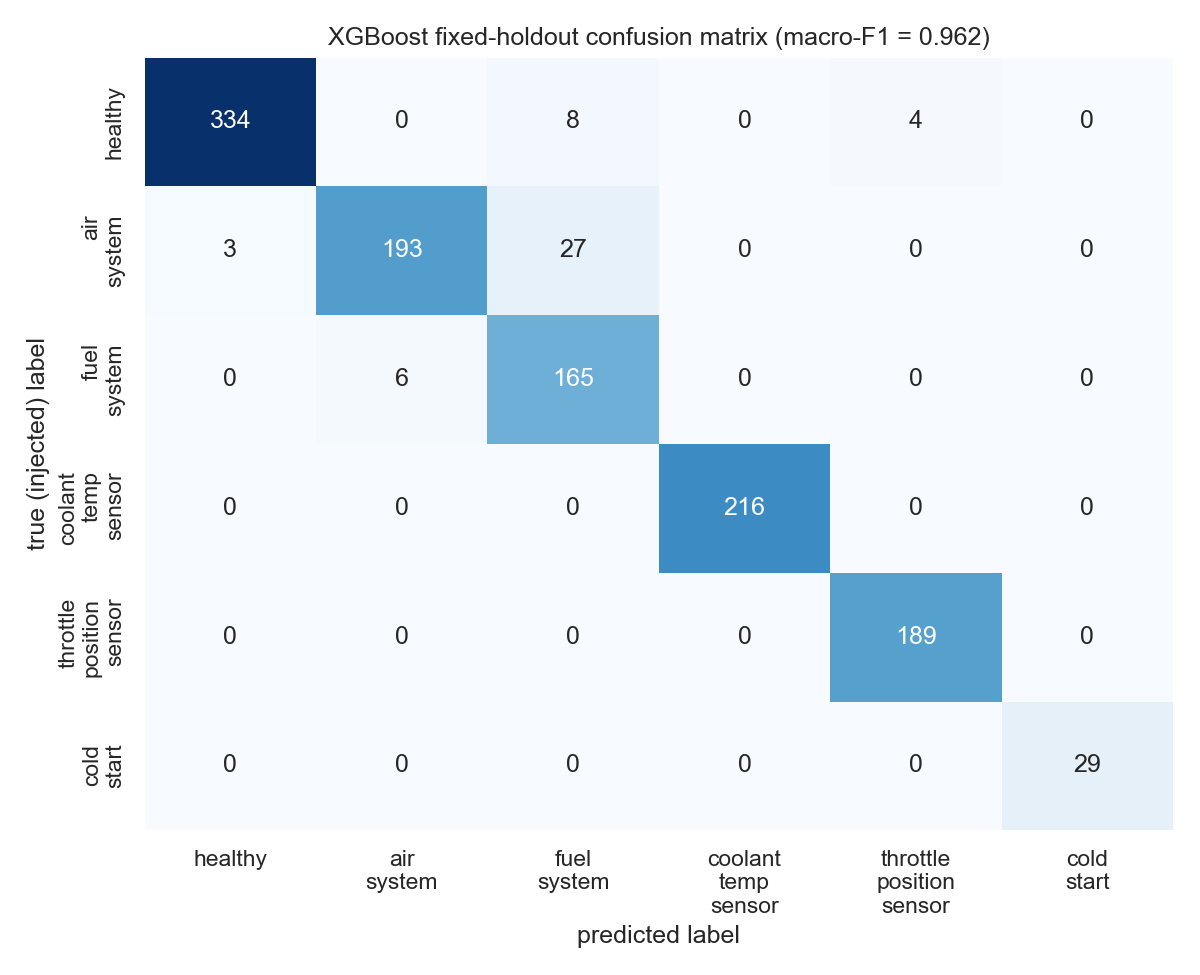
\includegraphics[width=0.85\textwidth]{fig_confusion_xgb.png}
  \caption{Fixed-holdout confusion matrix for the six-class XGBoost
    classifier (sessions drive1 + live12; macro-F1 = 0.962).}
  \label{fig:confusion}
\end{figure}

Figure~\ref{fig:confusion} shows where the errors live: almost entirely
inside a healthy--air--fuel triangle. The largest single cell is
air\_system predicted as fuel\_system (27 of 223 air windows), with smaller
flows of healthy into fuel (8) and fuel into air (6). The triangle is
physically sensible. Early-ramp air and fuel faults both surface first as
small fuel-trim disturbances at idle, and a window straddling the fault
onset is legitimately ambiguous between ``still healthy'' and ``barely
faulty.'' Coolant-sensor and cold-start windows, whose thermal signatures
are unambiguous at 1\,Hz, are never confused with anything (F1 = 1.000 and
support 216 and 29 respectively).

\subsection{Data Exploration Results}
\label{sec:eda}

The exploratory analysis below was produced by the repository's Phase-1
notebook against the recovered 129-file corpus; the figure-generation
script in \texttt{docs/book/figures/} reproduces every plot.

\begin{figure}[H]
  \centering
  \begin{subfigure}{0.48\textwidth}
    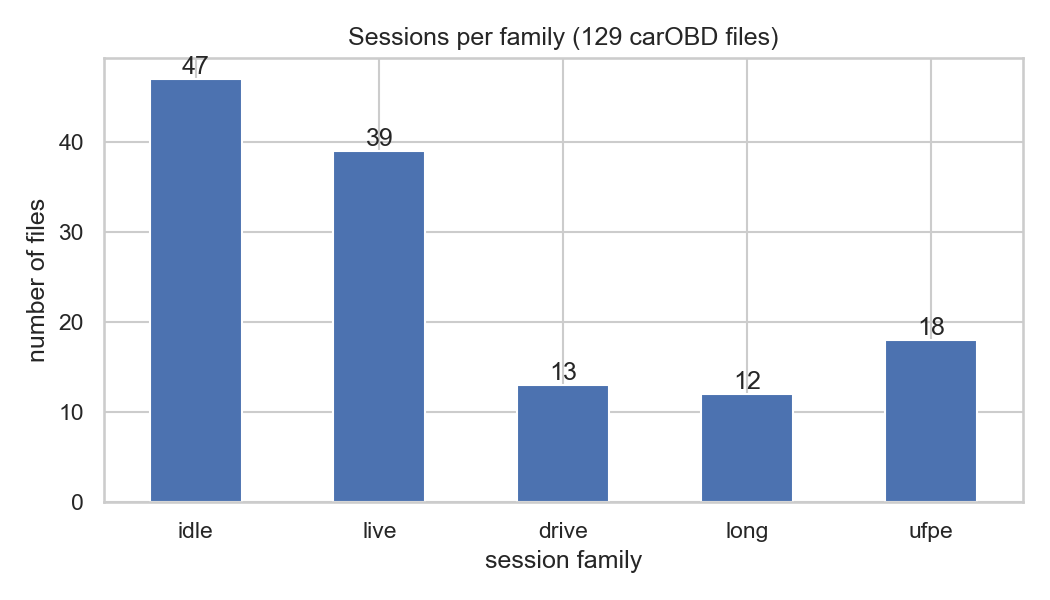
\includegraphics[width=\textwidth]{fig_family_sessions.png}
    \caption{Sessions per family.}
    \label{fig:families}
  \end{subfigure}
  \hfill
  \begin{subfigure}{0.48\textwidth}
    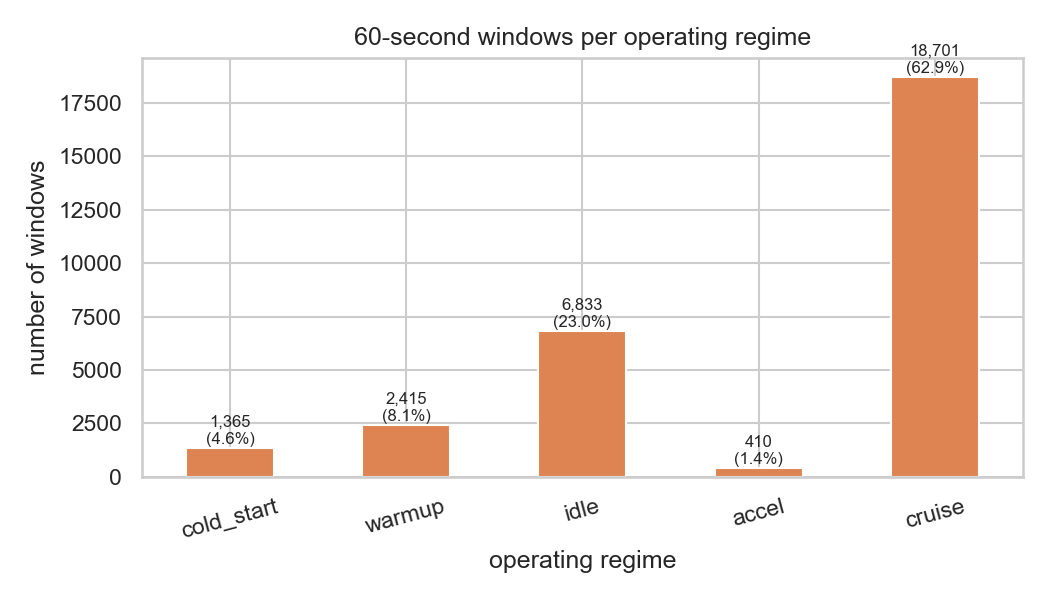
\includegraphics[width=\textwidth]{fig_regime_windows.png}
    \caption{Windows per operating regime.}
    \label{fig:regimes}
  \end{subfigure}
  \caption{Corpus composition on both axes. By file count the idle family
    dominates (47 of 129); by 60-second windows, cruise dominates (62.9\,\%)
    because driving sessions are far longer than idle ones.}
  \label{fig:composition}
\end{figure}

Composition is imbalanced on both axes, and the two axes disagree
(Figure~\ref{fig:composition}). Idle recordings are the most numerous
\emph{files}, but cruise dominates the \emph{window} count at 62.9\,\%,
followed by idle at 23.0\,\%, warm-up at 8.1\,\%, cold-start at 4.6\,\%,
and acceleration at just 1.4\,\%. The scarce regimes matter
disproportionately: a TPS fault only expresses under pedal load, and
cold-start windows are the entire training basis for that class. Class
balancing at training time addresses the label imbalance; the accel-regime
scarcity is a property of 60-second windows over real driving that
balancing cannot fix.

\begin{figure}[H]
  \centering
  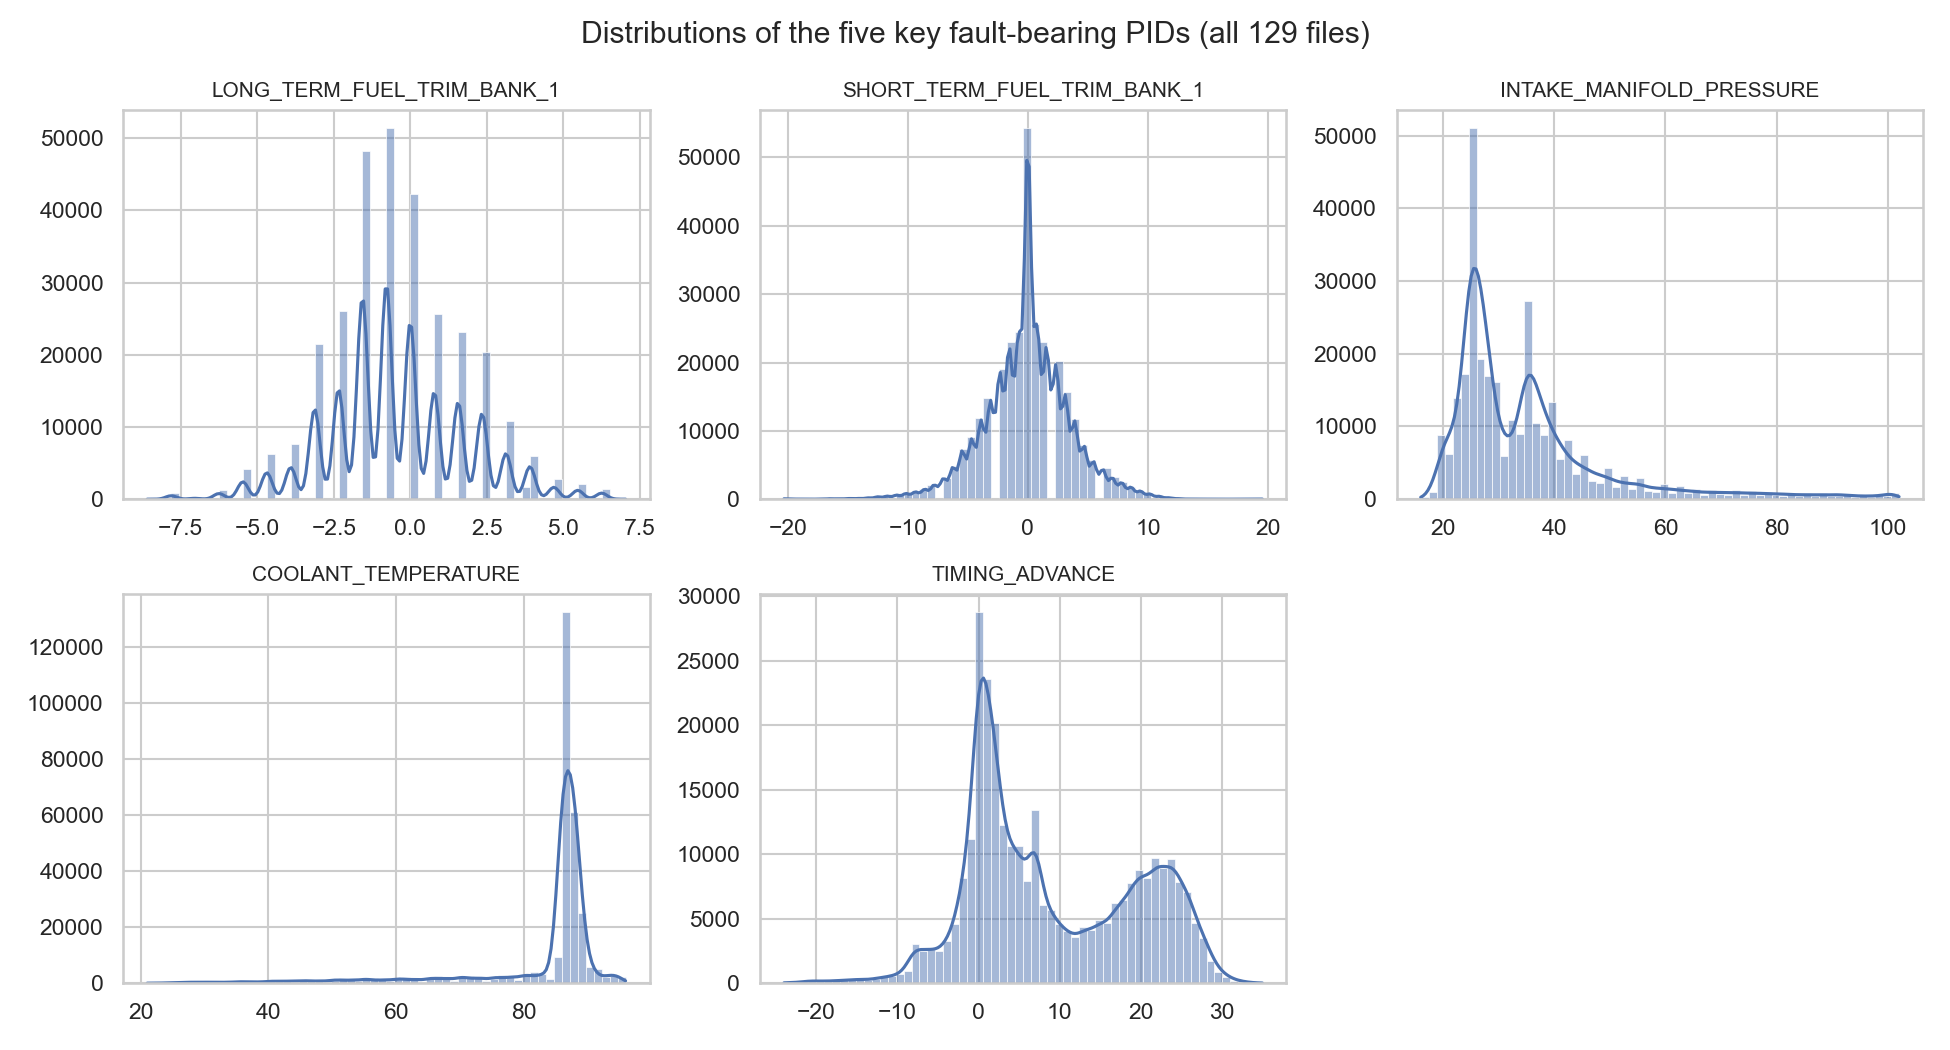
\includegraphics[width=\textwidth]{fig_fault_pid_distributions.png}
  \caption{Distributions of the five key fault-bearing PIDs across all 129
    files. Fuel trims are roughly symmetric and slightly rich-shifted with
    visible OBD-II quantization; coolant is bimodal (cold-start shoulder
    plus a warm-operation peak near 88--90$^{\circ}$C); MAP is multimodal
    from the idle/driving mixture; timing sits entirely inside its physical
    envelope.}
  \label{fig:distributions}
\end{figure}

The distribution shapes (Figure~\ref{fig:distributions}) argue for the
pipeline's normalization choice: multimodal, skewed channels do not reward
any Gaussian assumption on raw values, whereas per-vehicle z-scoring
measures displacement from the car's own mixture. The coolant bimodality
confirms cold-start data is well represented, and the timing histogram ---
bounded in $[-24^{\circ}, +35^{\circ}]$ across the entire corpus --- is
the standing proof that the column-shift repair holds
(Figure~\ref{fig:timingfix} showed the same channel reaching
776.6$^{\circ}$ under the defective parse).

\begin{figure}[H]
  \centering
  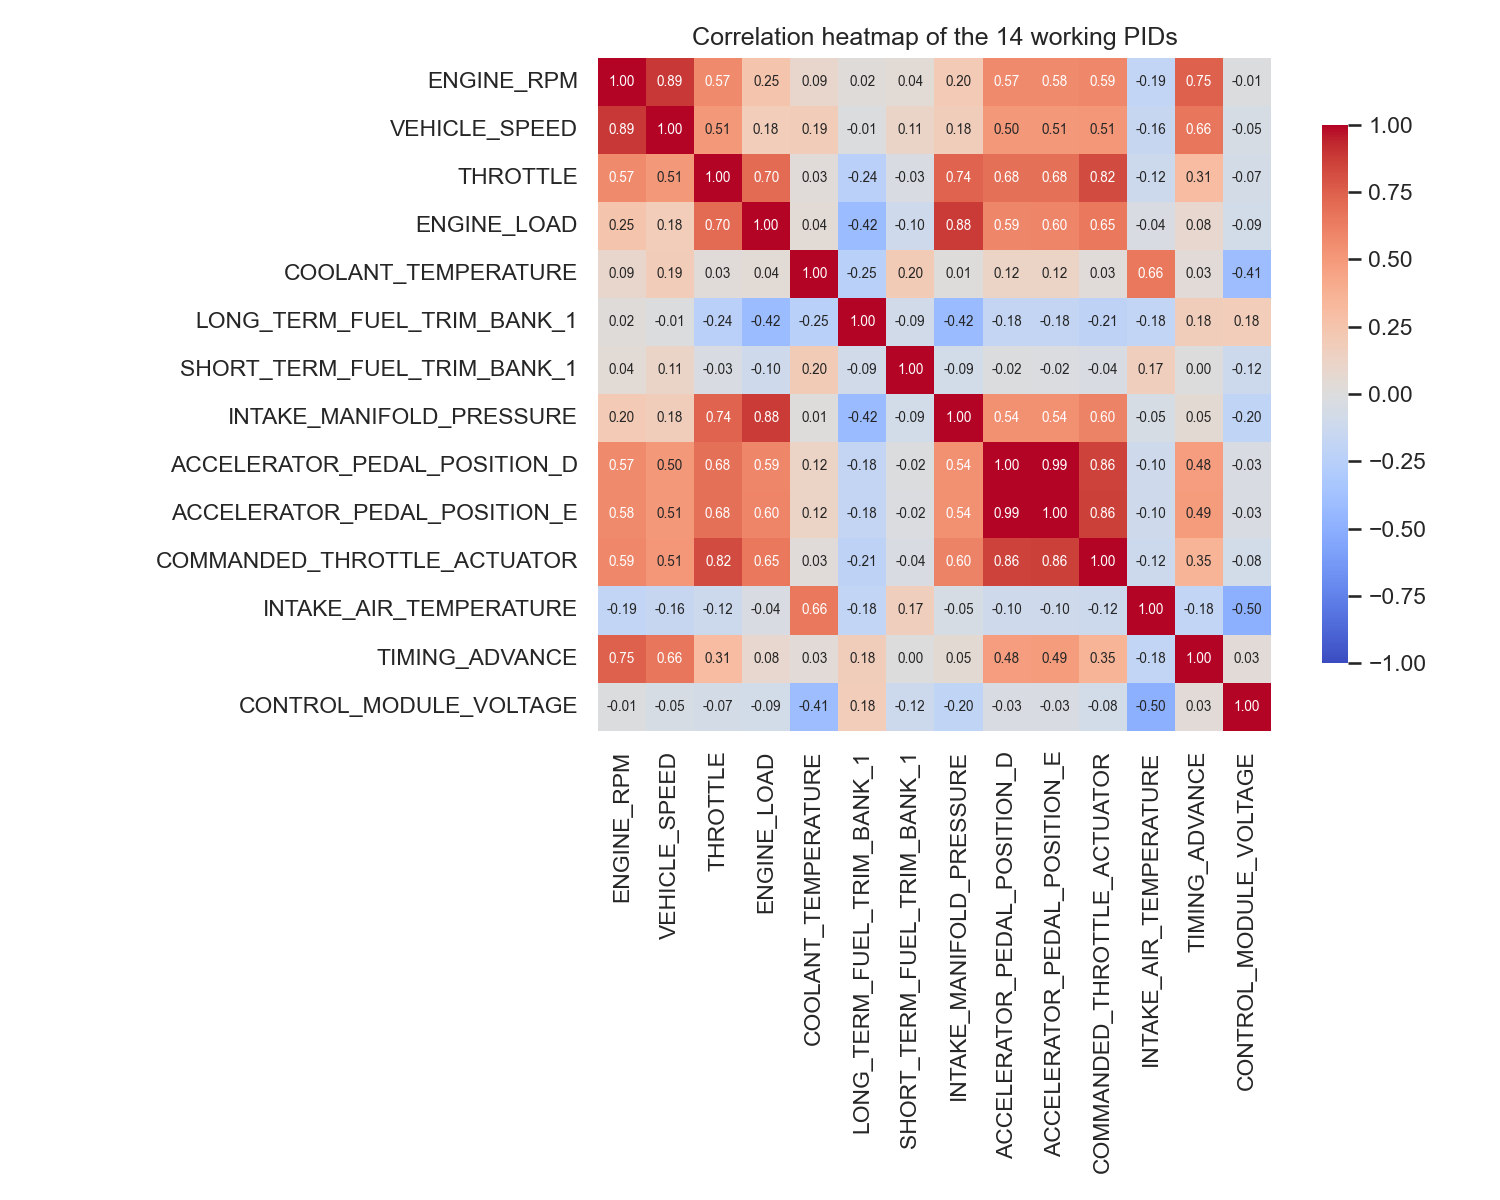
\includegraphics[width=0.9\textwidth]{fig_corr_heatmap.png}
  \caption{Correlation heatmap of the 14 working PIDs over the full corpus.}
  \label{fig:corr}
\end{figure}

The correlation structure (Figure~\ref{fig:corr}) shows the expected
physical couplings --- RPM with speed, MAP with engine load, and a tight
throttle/pedal cluster in which the two accelerator-pedal channels are
near-duplicates of each other. We keep both pedal channels despite the
redundancy: their \emph{agreement} is exactly what a TPS fault disturbs,
and the availability contract of Section~\ref{sec:dashboard} treats them as
jointly required for that class.

\begin{figure}[H]
  \centering
  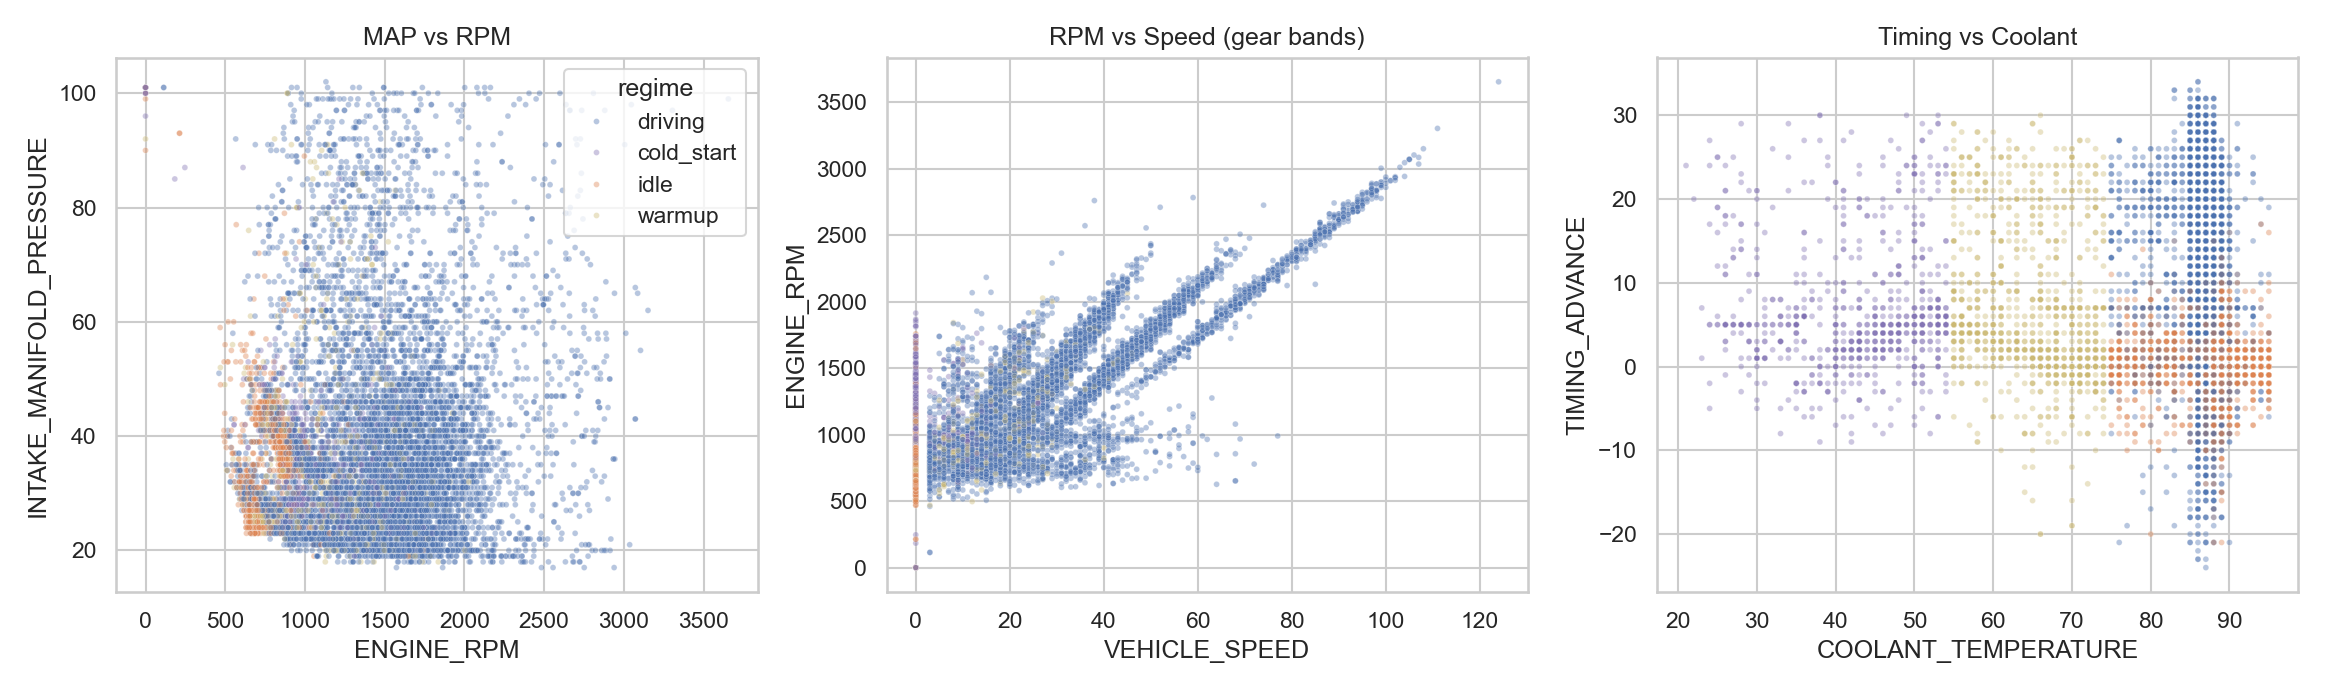
\includegraphics[width=\textwidth]{fig_bivariate.png}
  \caption{Bivariate structure, colored by a row-level regime proxy.
    Left: MAP vs RPM separates the idle cluster from the driving cloud ---
    the region the air-system fault perturbs. Center: RPM vs speed resolves
    into discrete gear bands, a drivetrain sanity check that a residual
    column shift would scramble. Right: timing advance climbs and
    stabilizes as coolant warms --- the coupling the coolant-sensor fault
    exploits.}
  \label{fig:bivariate}
\end{figure}

The bivariate views (Figure~\ref{fig:bivariate}) close the loop between
data and fault design: three of the four injected signatures are visible as
structure in the healthy data itself. Clean gear rays in the center panel
across all 129 files are also the most legible visual proof that the
recovered corpus is physically coherent. Duplicate rows, at 29{,}329
(9.6\,\%), are dominated by legitimate steady-state repeats at 1\,Hz ---
an idling engine reports the same values for many consecutive seconds ---
so we do not drop them; deleting idle repeats would distort exactly the
statistics the idle-gated air-system model depends on.

\subsection{Real-Vehicle Testing}
\label{sec:realvehicle}

The deployment target was a healthy 2015 Toyota Yaris --- a different car,
a different engine-management philosophy (MAF-based), and a different
decade from the training vehicle. Data reached the pipeline through the
OBD-LOG app and an ELM327 Bluetooth adapter. We scored two recordings:
\texttt{obd22}, a 1{,}740-row (29-minute at 1\,Hz) session used as the
baseline capture, and \texttt{transition}, a 2{,}148-row session spanning a
cold start and the transition into driving. The app's three tier captures
(124, 121, and 65 rows at parked idle) served as the throughput tests of
Table~\ref{tab:pollrate}.

The single missing channel dominates everything about this test. On both
recordings, exactly one working PID is absent: \texttt{INTAKE\_MANIFOLD\_%
PRESSURE}. The Yaris meters air with a MAF sensor and simply does not
expose PID 010B, so the MAP column is present in the CSV schema but empty
in every row.

\begin{table}[H]
  \centering
  \caption{Real-vehicle scoring outcomes on the healthy 2015 Toyota Yaris,
    with the Untested contract applied. Raw label counts are the
    classifier's per-window outputs before suppression.}
  \label{tab:yaris}
  \begin{tabular}{lcccc}
    \toprule
    Session & Rows / windows & Missing PIDs & Evaluable windows & Verdict\\
    \midrule
    obd22      & 1{,}740 / 169 & MAP only & 7 of 169 & INSUFFICIENT DATA\\
    transition & 2{,}148 / 209 & MAP only & 6 of 209 & INSUFFICIENT DATA\\
    \bottomrule
  \end{tabular}
\end{table}

Behind Table~\ref{tab:yaris} sits the incident that reshaped the system.
Before the Untested contract existed, missing MAP features were filled with
the \emph{training vehicle's} baseline values. To the classifier, a
perfectly flat, perfectly average MAP on a car whose every other channel
varied normally looked like an enormous deviation --- and the model mapped
that artifact squarely onto air\_system. The healthy Yaris scored
``97\,\% air\_system, FAULT DETECTED.'' The raw label counts still show the
shape of that failure: on \texttt{obd22}, 162 of 169 windows carry the
air\_system label (with 5 healthy, 1 fuel, 1 TPS); on \texttt{transition},
203 of 209. Fabricated sensor values produce confident wrong answers ---
that is the design lesson we consider this test's main deliverable.

With the contract in place, the same recordings produce the correct
behavior end to end: MAP-dependent features stay NaN, air\_system is
declared Untested for the session, its windows are excluded from
evaluation, and the seven (respectively six) remaining evaluable windows
fall below the ten-window floor --- so the report prints INSUFFICIENT
EVALUABLE DATA instead of a verdict. We want to be precise about what this
outcome is: it is not a failed test. The system was shown a car it cannot
fully evaluate and said so, where its predecessor invented a fault. On a
MAF-based car, honest air-system coverage requires a MAF-based feature
path, and that is future work, not a rounding error.

The channels that \emph{were} available behaved healthily. LTFT sat at
$-6.4\,\%$ mean (spread $-8.3$ to $-4.5\,\%$) across the Yaris recordings
--- a mild, steady rich bias, consistent across sessions, comfortably
inside the $\pm10\,\%$ band that our fuel-fault severity model treats as
the concern threshold, and exactly the kind of per-vehicle personality the
baseline z-scoring exists to absorb.

\subsection{Forecaster Results}
\label{sec:forecastresults}

Table~\ref{tab:forecaster} evaluates the four PID-forecaster regressors
against the persistence baseline (``the next 60 seconds change nothing''),
in z-scored units on held-out sessions.

\begin{table}[H]
  \centering
  \caption{PID forecaster mean absolute error (z-units, 60\,s horizon,
    held-out sessions) versus the persistence baseline.}
  \label{tab:forecaster}
  \begin{tabular}{lccc}
    \toprule
    Target channel & Forecaster MAE & Persistence MAE & Beats baseline?\\
    \midrule
    COOLANT\_TEMPERATURE      & 0.050 & 0.112 & Yes (2.3$\times$ better)\\
    INTAKE\_MANIFOLD\_PRESSURE & 0.773 & 0.800 & Barely\\
    THROTTLE\_TO\_PEDAL\_RATIO & 0.829 & 0.903 & Barely\\
    LONG\_TERM\_FUEL\_TRIM     & 1.152 & 0.492 & \textbf{No --- 2.3$\times$ worse}\\
    \bottomrule
  \end{tabular}
\end{table}

The pattern is physical. Coolant temperature follows slow, deterministic
thermal dynamics, and the forecaster genuinely learns them. MAP and the
throttle-to-pedal ratio are driver-driven; sixty seconds ahead, the driver
is close to unpredictable, and the forecaster only marginally beats
assuming nothing happens. LTFT is the painful row: its 60-second change on
healthy data is near-zero noise around a session-specific level, the model
overreacts to that noise, and it loses to persistence by a factor of 2.3
--- on the one channel most diagnostic of fuel faults. We keep the LTFT
regressor in the artifact set and its failure in this table, because a
reader who deploys Pillar~2 must know that the drift signal for fuel
faults comes from the anomaly detector and the classifier, not from the
forecaster. For completeness, the one-class IsolationForest scores an AUC
of 0.69 (95\,\% CI 0.66--0.72) separating healthy from any-fault windows
on the synthetic test set, and its false-positive rate on held-out healthy
sessions (15.6\,\% at the intended 1\,\% budget) is the measured argument
for per-vehicle re-fit before any live use.

\subsection{Discussion}

Three threads run through these results. First, the evaluation hierarchy
did its job: the same model that scores 1.000 (RF) or 0.962 (fixed holdout)
under leaky-adjacent conditions scores 0.699 on its worst honest fold, and
designing the report around the floor rather than the ceiling changed what
we were willing to claim. Second, the cross-vehicle test produced no
detection result at all --- and that non-result, delivered as two correct
refusals on a car the first version had confidently mislabeled, is the
strongest evidence in this book that the reporting layer works. Third,
every number above is bounded by the same asterisk: the faults were written
by our own injector. The 0.033 withheld-configuration gap says the model is
not merely memorizing coefficients; nothing in this chapter says it detects
real faults. Closing that gap needs data, not modeling, and
Section~\ref{sec:future} puts it first in line accordingly.

Read together, the classification results, the forecaster failure on LTFT,
and the Yaris deployment tell a consistent story rather than three separate
ones. Wherever a signal is slow and thermally or mechanically determined
--- coolant warm-up, timing versus temperature --- both the classifier and
the forecaster do well, because the underlying physics leaves little room
for session-specific noise to hide in. Wherever a signal reflects the
ECU's learned, car-specific fuel state --- LTFT above all --- both
components struggle, because the same absolute trim value means something
different on every car and every tank of fuel. That split is not a
coincidence of which experiments happened to work; it is the same physical
fact showing up three separate times, and it is the strongest argument in
this report for treating per-vehicle baselining as necessary rather than
optional.

\clearpage
\section{Conclusion and Future Work}
\label{ch:conclusion}

\subsection{Conclusions}

We set out to catch a developing engine fault from the standard 1\,Hz
OBD-II stream, before a diagnostic trouble code fires. What we built is a
physics-grounded fault injection engine for four common fault classes; a
vehicle-agnostic feature and normalization pipeline that lets a model
trained on one car run on another; a six-class XGBoost classifier evaluated
under session-level and family-level cross-validation; a per-PID
forecaster and a one-class anomaly detector as a second, independent line
of evidence; a native Android application, OBD-LOG, for real-vehicle data
collection over Bluetooth; a live Streamlit dashboard that explains its own
predictions and closes every session with a plain-language health verdict;
and, threaded through all of it, a reporting layer that says ``Untested''
or ``insufficient data'' instead of manufacturing a number it cannot back.

What we did not build is a validated real-fault detector. That distinction
matters more than any F1 score in this book, and we have tried not to blur
it anywhere above. Every classification number in Chapter~\ref{ch:results}
measures the model's ability to recover labels written by our own
injector. Building the validated version needs one thing our project could
not supply on its own timeline: labeled recordings of real, induced faults.
Section~\ref{sec:future} makes that the first line of future work, not the
last, because it is the single change that would do the most.

If this project has one engineering contribution worth naming beyond the
models themselves, it is the discipline of refusal. Twice in this book the
system was handed a situation it could not honestly resolve --- a vehicle
missing the sensor a fault class depends on, a recording too short to
support a verdict --- and twice it said so instead of guessing. The
alternative version of this system, the one we shipped first and then
un-shipped, guessed with 97\,\% confidence on a healthy car. We consider the
version that admits what it does not know to be the more useful tool, even
though it produces fewer confident-looking numbers for a slide.

That discipline did not come free. It cost us a working demo we had to
throw away, a redesign of the reporting layer around an evaluability
contract nobody had asked for at project kickoff, and an uncomfortable
week of explaining to each other why a 97\,\% confidence score was the
project's worst result rather than its best. We record that cost here
because a reader building a similar system will hit the same choice ---
ship the number the model gives you, or build the machinery to know when
that number is not trustworthy --- and the second path is more work for a
less impressive-looking demo. We think it is the only defensible path for
anything a mechanic or a driver might actually act on.

The broader lesson carries past this particular car and these particular
four faults. Any system trained on synthetic labels inherits the honesty
of its label generator, and any system deployed across more than one
instance of its target domain inherits the assumptions baked into its
first training example. We tried to make both of those inheritances
visible rather than implicit: the injector's physics reasoning lives next
to its code, the withheld-configuration gap is a number in this book and
not a footnote, and the cross-vehicle failure that produced the Untested
contract is documented as a failure, not smoothed into a success story
after the fact. If a future team extends this work, we would rather they
inherit the visible assumptions than have to rediscover them the way we
did.

\subsection{Limitations}

We list these without softening them, because the audience for this report
already knows the honest framing and overselling would cost more credibility
than it could ever buy back.

\begin{enumerate}
  \item \textbf{Every fault metric in this book measures self-consistency,
    not field performance.} The injector writes the fault; the classifier
    learns to invert the injector. A macro-F1 of 0.958 on a held-out
    driving family says the model generalizes across driving contexts for
    faults it was told to recognize. It does not say the model would catch
    a real vacuum leak on a real car. No experiment in this project
    contradicts that limitation, and none was designed to.
  \item \textbf{The model has never detected a real fault.} Not once, on
    any vehicle, in any recording. The real-fault evaluation code exists
    in the repository and its data folder is empty. This is the single
    most important gap between what we built and what a mechanic would need
    to trust it.
  \item \textbf{Air-system detection is unavailable on the majority of
    modern cars.} MAF-based engines --- our own test vehicle among them ---
    expose no MAP sensor, and the air-system fault's primary signature
    lives on MAP. On those cars the class is correctly marked Untested, but
    correctly refusing to answer is not the same as answering.
  \item \textbf{Phone-based sampling aliases fast dynamics.} Our measured
    ELM327 poll rate falls to 0.37\,Hz at 21 polled PIDs --- well under the
    1\,Hz the training pipeline assumes. Results scored on app-captured
    data should be read as pessimistic relative to a faster logger, because
    slow polling smears short fuel-trim oscillations into apparent
    stability, which can understate real trim variance and, in the other
    direction, overstate false-positive risk on transient events the
    sampler simply missed.
  \item \textbf{Self-baselining cannot see a fault that predates the
    recording.} The end-of-read report treats the first 20\,\% of a session
    as healthy ground truth. A car that is already faulty at key-on has
    that fault baked into its own baseline and will read as normal for the
    rest of the drive. This is a structural property of the self-baseline
    design, not a bug to be patched.
\end{enumerate}

\subsection{Future Work}
\label{sec:future}

The items below are ordered by impact, not by how soon they could be
started. Each one names a specific mechanism and a specific reason it was
not already done, because ``improve the model further'' is not a plan.

\begin{enumerate}
  \item \textbf{Real fault data.} This is the one change that would convert
    the project from ``a detection algorithm plus a collection protocol''
    into a validated detector. A single matched set of before, during, and
    after recordings of a genuinely induced fault --- a vacuum line
    partially disconnected under a mechanic's supervision, say --- would let
    the real-fault evaluation code that already exists in the repository
    produce its first non-empty result. We did not do this in the current phase
    because it requires a donor vehicle, a supervising mechanic, and a
    written abort protocol we were not yet in a position to execute safely;
    the collection protocol documenting exactly how to do it is already
    written and waiting in the repository, alongside the scorer that would
    consume its output.

  \item \textbf{A live Android-to-server pipeline.} Route the app's CSV
    output over HTTPS, in roughly 60-second chunks, to a cloud-hosted
    version of the existing FastAPI backend, which already implements JWT
    authentication. The server holds one persistent scoring session per
    vehicle --- one fitted baseline, every chunk scored against it in
    sequence --- and the Streamlit dashboard mirrors that session live
    while the phone shows a simplified health card. This was not built now
    because it needs a hosting decision (which cloud, which uptime
    guarantee) that is out of scope for a laptop-based thesis defense, and
    because it depends on item 1 producing enough real sessions to be
    worth streaming.

  \item \textbf{Apache Kafka for multi-vehicle ingest.} At fleet scale,
    direct HTTP ingest does not survive a phone losing signal mid-upload,
    and a new server process per vehicle does not scale. The natural next
    architecture makes the Android app a Kafka producer, runs a consumer
    group that performs inference per vehicle, and writes a second consumer
    to a time-series store for the dashboard to query. Kafka's offset-based
    replay absorbs cellular dropouts that a plain HTTP POST cannot, and a
    Kafka Connect OBD-II source connector is the natural long-term target.
    This is future work rather than current work because it only pays for
    itself once item~2 exists and more than one or two vehicles are
    actually streaming --- building it first would be premature
    infrastructure for a single-laptop demo.

  \item \textbf{Per-regime baselining.} Right now one healthy baseline
    covers idle and driving alike, and we measured the resulting
    idle-to-drive feature shift at a mild 2--3$\sigma$, concentrated on the
    throttle side, and already absorbed by the regime one-hot features and
    the alerter's temporal vote. Because the measured shift is mild, this
    is a robustness improvement queued behind the higher-impact items
    above, not a critical bug demanding an emergency fix. Implementing it
    properly means retraining with regime-conditioned normalization rather
    than patching the existing scaler.

  \item \textbf{Intermittent and accelerating fault shapes in the
    injector.} Every fault the injector produces today follows one shape:
    a linear ramp to a held plateau. Real components do not always fail
    that way --- a connector that only opens under vibration produces an
    intermittent signature, and bearing-style wear often follows a
    Weibull-shaped acceleration rather than a straight line. Widening the
    injector's shape library would reduce the risk that the classifier is
    quietly overfitting to ``ramp-then-hold'' as a pattern rather than
    learning the underlying fault physics. We scoped this out of the
    current phase because the four existing fault models, in ramp and step
    mode, already consumed the available time for physics validation, and
    adding shapes without re-validating physics for each one would
    reintroduce exactly the kind of unaudited synthetic data this project
    was built to avoid.

  \item \textbf{A session-label field in the Android app.} A single text
    field, written as one more CSV column, so a recording can declare
    itself \emph{baseline}, \emph{fault-type-X}, or \emph{healthy-post-repair}
    without an external notebook tracking which file is which. It is a
    small UI change, deliberately left until last because it only becomes
    necessary once real-fault collection (item~1) is actually underway ---
    there is no annotation burden to solve before then.
\end{enumerate}

\clearpage

% ═══════════════════ REFERENCES ═══════════════════
\bibliographystyle{IEEEtran}
\bibliography{references}
\clearpage

% ═══════════════════ APPENDICES ═══════════════════
\appendix

\section{Key Source Code Listings --- Analysis Pipeline}
\label{app:python}

The listings below are included verbatim from the project repository
(\texttt{Predictive-MaintenanceV1}) at the revision this book was built
from. They are the four modules the main text leans on most: the fault
injection engine (Section~\ref{sec:injector}), the XGBoost training module
(Section~\ref{sec:models}), the end-of-read session report
(Section~\ref{sec:dashboard}), and the PID availability contract that
implements the Untested behavior.

\lstinputlisting[style=pystyle,
  caption={\texttt{src/injection/fault\_injector.py} --- the
    physics-constrained fault injection engine.},
  label={lst:injector}]{../../src/injection/fault_injector.py}

\clearpage
\lstinputlisting[style=pystyle,
  caption={\texttt{src/models/xgb\_classifier.py} --- XGBoost training,
    evaluation, and persistence, including class-balance weights and the
    fuel-system down-weight.},
  label={lst:xgb}]{../../src/models/xgb_classifier.py}

\clearpage
\lstinputlisting[style=pystyle,
  caption={\texttt{src/eval/session\_report.py} --- the end-of-read health
    report: 20\,\% self-baseline, physics-severity 95th percentile,
    inconclusive rule, and the minimum-evaluable-windows floor.},
  label={lst:report}]{../../src/eval/session_report.py}

\clearpage
\lstinputlisting[style=pystyle,
  caption={\texttt{src/eval/pid\_availability.py} --- per-fault required
    PIDs and the Untested contract.},
  label={lst:pidavail}]{../../src/eval/pid_availability.py}

\clearpage
\section{Key Source Code Listings --- OBD-LOG Android App}
\label{app:android}

The two listings below are copied from the OBD-LOG repository
(\texttt{github.com/Terminatorbds/OBD-LOG}), from
\texttt{app/src/main/java/com/example/obdlogger/}. \texttt{ObdPids.kt}
defines the tiered PID table and the reply parser;
\texttt{ObdLogger.kt} performs ELM327 initialization, ECU capability
detection via the support bitmasks, and single-PID reads.

\lstinputlisting[style=ktstyle,
  caption={\texttt{ObdPids.kt} --- tiered PID definitions, decode formulas,
    and ELM327 reply parsing.},
  label={lst:obdpids}]{listings/ObdPids.kt}

\clearpage
\lstinputlisting[style=ktstyle,
  caption={\texttt{ObdLogger.kt} --- adapter initialization and
    supported-PID detection.},
  label={lst:obdlogger}]{listings/ObdLogger.kt}

\clearpage
\section{Full Per-Class Metrics Tables}
\label{app:metrics}

All values below are taken directly from the evaluation artifacts in the
repository's \texttt{results/} directory
(\texttt{xgb\_classifier\_v1\_results.json}, \texttt{lofo\_eval.json},
\texttt{loso\_cv\_results.json}, \texttt{rf\_classifier\_v1\_results.json},
\texttt{withheld\_coeff\_results.json}).

\begin{table}[H]
  \centering
  \caption{XGBoost fixed-holdout (drive1 + live12) per-class metrics.
    Macro-F1 = 0.962.}
  \label{tab:xgbperclass}
  \begin{tabular}{lcccc}
    \toprule
    Class & Precision & Recall & F1 & Support\\
    \midrule
    healthy                    & 0.991 & 0.965 & 0.978 & 346\\
    air\_system                & 0.970 & 0.865 & 0.915 & 223\\
    fuel\_system               & 0.825 & 0.965 & 0.889 & 171\\
    coolant\_temp\_sensor      & 1.000 & 1.000 & 1.000 & 216\\
    throttle\_position\_sensor & 0.979 & 1.000 & 0.990 & 189\\
    cold\_start                & 1.000 & 1.000 & 1.000 & 29\\
    \bottomrule
  \end{tabular}
\end{table}

\begin{table}[H]
  \centering
  \caption{Random Forest baseline, fixed holdout, earlier five-class task.
    Macro-F1 = 1.000 --- reported as a memorization warning, not a result.}
  \label{tab:rfperclass}
  \begin{tabular}{lcccc}
    \toprule
    Class & Precision & Recall & F1 & Support\\
    \midrule
    healthy                    & 1.000 & 1.000 & 1.000 & 375\\
    air\_system                & 1.000 & 1.000 & 1.000 & 163\\
    fuel\_system               & 1.000 & 1.000 & 1.000 & 163\\
    coolant\_temp\_sensor      & 1.000 & 1.000 & 1.000 & 163\\
    throttle\_position\_sensor & 1.000 & 1.000 & 1.000 & 163\\
    \bottomrule
  \end{tabular}
\end{table}

\begin{table}[H]
  \centering
  \caption{LOFO cross-validation: per-class F1 for every held-out family.
    Mean macro-F1 = 0.977, $\sigma$ = 0.012.}
  \label{tab:lofofull}
  \begin{tabular}{lccccc}
    \toprule
    & \multicolumn{5}{c}{Held-out family}\\
    \cmidrule(lr){2-6}
    Class & drive & idle & live & long & ufpe\\
    \midrule
    healthy                    & 0.968 & 0.933 & 0.933 & 0.983 & 0.984\\
    air\_system                & 0.989 & 0.980 & 0.965 & 0.988 & 0.989\\
    fuel\_system               & 0.995 & 0.991 & 0.917 & 0.989 & 0.978\\
    coolant\_temp\_sensor      & 1.000 & 0.999 & 1.000 & 1.000 & 1.000\\
    throttle\_position\_sensor & 0.951 & 0.910 & 0.932 & 0.969 & 0.972\\
    cold\_start                & 0.995 & 1.000 & 1.000 & 1.000 & 1.000\\
    \midrule
    Macro-F1                   & 0.983 & 0.969 & 0.958 & 0.988 & 0.987\\
    Test windows               & 12{,}568 & 21{,}802 & 30{,}336 & 19{,}270 & 10{,}454\\
    Test sessions              & 13 & 47 & 39 & 12 & 18\\
    \bottomrule
  \end{tabular}
\end{table}

\begin{table}[H]
  \centering
  \caption{LOSO cross-validation summary over all 129 single-session folds.}
  \label{tab:losofull}
  \begin{tabular}{lc}
    \toprule
    Statistic & Macro-F1\\
    \midrule
    Mean               & 0.917\\
    Standard deviation & 0.084\\
    Best fold          & 1.000 (multiple sessions)\\
    Worst fold         & 0.699 (live31)\\
    \bottomrule
  \end{tabular}
\end{table}

\begin{table}[H]
  \centering
  \caption{Withheld-configuration experiment: train on injector
    configuration A, evaluate on configuration B.}
  \label{tab:withheld}
  \begin{tabular}{lcc}
    \toprule
    & Config A (train) & Config B (withheld)\\
    \midrule
    air\_system magnitude (kPa-eq.)       & 13.0 & 9.0\\
    fuel\_system magnitude (\% LTFT)      & 18.0 & 24.0\\
    coolant\_temp\_sensor target ($^{\circ}$C) & 42.0 & 38.0\\
    throttle\_position\_sensor factor     & 1.35 & 1.50\\
    Onset fraction                        & 0.40 & 0.55\\
    Ramp fraction                         & 0.15 & 0.25\\
    Noise $\sigma$                        & 0.3  & 0.5\\
    \midrule
    Macro-F1                              & 0.892 & 0.859\\
    \multicolumn{3}{l}{Gap = 0.033 (same-config minus withheld-config)}\\
    \bottomrule
  \end{tabular}
\end{table}


\end{document}
